\documentclass[12pt,a4paper,oneside]{report}

% ---- Fonts (compile with XeLaTeX or LuaLaTeX: the text uses IAST diacritics) ----
\usepackage{fontspec}
\setmainfont{TeX Gyre Termes}
\usepackage{amsmath,amssymb}
% Termes lacks a precomposed m-dot-above (U+1E41); build it from m + combining dot.
\usepackage{newunicodechar}
\newunicodechar{ṁ}{m\char"0307{}}

% ---- Page layout ----
\usepackage[a4paper,left=1.25in,right=1in,top=1in,bottom=1in]{geometry}
\usepackage{setspace}
\onehalfspacing
\usepackage{parskip}
\setlength{\emergencystretch}{3em}

% ---- Headings ----
\usepackage{titlesec}
\titleformat{\chapter}[hang]{\normalfont\LARGE\bfseries}{\thechapter.}{0.6em}{}
\titlespacing*{\chapter}{0pt}{0pt}{1.2em}
\titleformat{\section}{\normalfont\Large\bfseries}{\thesection}{0.8em}{}
\titleformat{\subsection}{\normalfont\large\bfseries}{\thesubsection}{0.8em}{}
\setcounter{secnumdepth}{2}
\setcounter{tocdepth}{2}

% ---- Tables, figures, links ----
\usepackage{longtable,booktabs,array,calc}
\usepackage{graphicx}
\usepackage[font=small,labelfont=bf]{caption}
\usepackage{xcolor}
\usepackage{xurl}
\usepackage[numbers,sort&compress]{natbib}
\usepackage[hidelinks,unicode]{hyperref}
\usepackage{bookmark}
\newcommand{\doi}[1]{\href{https://doi.org/#1}{doi:#1}}
\usepackage{titlecaps}
% ---- Header/footer ----
\usepackage{fancyhdr}
\pagestyle{fancy}
\fancyhf{}
\fancyfoot[C]{\thepage}
\renewcommand{\headrulewidth}{0pt}
\fancypagestyle{plain}{\fancyhf{}\fancyfoot[C]{\thepage}\renewcommand{\headrulewidth}{0pt}}

% ---- Report metadata ----
\newcommand{\reporttitle}{Computational Implementation of the Surya Siddhanta Across Fourteen Chapters}
\newcommand{\authorname}{Ashutosh Nigam}
\newcommand{\rollno}{M25AI2006}
\newcommand{\degree}{M.Tech.}
\newcommand{\supervisor}{Dr.\ Dinesh Mohan Joshi}
\newcommand{\institute}{Indian Institute of Technology Jodhpur}
\newcommand{\department}{Department of Computer Science and Engineering}
\newcommand{\submissiondate}{November 2026}

% Name of the text, used throughout the report
\usepackage{xspace}
\newcommand{\surya}{Sūrya Siddhānta\xspace}

\hypersetup{pdftitle={\reporttitle},pdfauthor={\authorname}}

\begin{document}

\pagenumbering{roman}

% ================= Abstract =================
\chapter*{Abstract}
\addcontentsline{toc}{chapter}{Abstract}

In this project, I implemented the computational methods of the \surya as a reusable Python library and built web and AI-based interfaces on top of it. Each of the text's fourteen chapters is its own module. Together they cover planetary motion and its corrections, eclipses, place and time calculations, conjunctions, stars, visibility, lunar phases, cosmography, astronomical instruments, and the calendar. The chapter-level functions do the actual astronomical calculations, and the React interfaces show the results along with references to the relevant parts of the source text.

The implementation uses \MakeUppercase{EBENEZER BURGESS}'s English translation, \MakeUppercase{\emph{A TEXT-BOOK OF HINDU ASTRONOMY WITH NOTES AND AN APPENDIX}} \cite{burgess1860}. I also checked calculations against worked examples in \MakeUppercase{MAHAVIR PRASAD SRIVASTAVA}'s Hindi book, \MakeUppercase{\emph{SURYA SIDDHANTA: VIGYAN BHASHYA}} \cite{shrivastava}. By using tests based on specific verses, along with examples written in the book, I found and fixed errors in the inner-planet calculations, the \emph{manda} anomaly, and the time calculations based on Ujjain.

I also built a separate project to extract the Hindi and English text from the source books. I tried several OCR models for this, and the processed text was used to build a searchable corpus. Right now the application includes all 500 numbered English verses from the fourteen chapters. The Hindi OCR output and its translations are kept separate and haven't been added to the same aligned corpus yet.

The main application is built using React and FastAPI. It lets users explore the chapters, follow eight learning paths, and use the Research Explorer. The AI chat interface can use either OpenRouter or DeepSeek as its conversational model, but the calculation results always come from the Python library. Finally, the project compares the \surya's longitude calculations with JPL DE440, using clearly defined conventions for date, time, and coordinates.

% ================= Contents =================
\tableofcontents

\clearpage
\pagenumbering{arabic}

\chapter{Introduction}

The \surya is an important classical Indian astronomical text written in Sanskrit~\cite{burgess1860, shrivastava,pandey_ss,plofker2009}. It describes mathematical methods for calculating the positions and motions of celestial bodies. The text includes rules for time measurement, planetary motion, eclipses and other astronomical phenomena. These rules provide a mathematical basis for several traditional Indian astronomical calculations~\cite{oak_week,ss_video}. The fourteen chapters start with measurement of time and mean planetary motions. Then it explains true positions, local geometry, eclipses, conjunctions, stars, visibility, the lunar crescent, instruments and calendar reckoning. A textual explanation of this may not explain all open question that what a quantity means or which clock or time a calculation uses. A working program can help to address this problem by displaying the calculated results with the parameters used.

In This project we also documented how the astronomical rules from the text are interpreted and implemented. For example a calculated longitude results requires an epoch and a coordinate convention. An eclipse calculation may require the observer's location depends on the type of eclipse and the quantities being calculated. The explanation derived from the text of book needs a chapter and verse reference from the book. With all these details, the reader can easily follow a calculation and question the choices behind it with explanations.

This project also supports the programmers who needs reusable functions and the readers who want to inspect the astronomical rules. Both programmers and readers needs to know whether a result is directly based on a verse or depends on an assumption made during implementation. So we added the chapter-based modules, verse references, and intermediate values which make it visible. This also helps reading and calculation interfaces share the same source references.

\chapter{Literature Survey}

\section{Source texts and editorial approach}

The main source for the astronomical rules and constants used in this project is the 1860 English translation of the \emph{\surya} by Ebenezer Burgess~\cite{burgess1860}. We also used examples from Mahavir Prasad Srivastava's Hindi \emph{\surya: Vigyan Bhashya}~\cite{shrivastava}. These examples provide intermediate values for specific dates and locations. They help in verifying the signs of calculated quantities, units and order of operations. I used Hindi OCR using multiple models to read the Hindi text from Vigyan Bhasya. Since OCR can confuse the nine and six of the period typeface so it was verified using Typed version of this book to check accuracy.

We mark where a procedure is following the verse and where it is following the commentary. This matters for the implementation in Chapter 13 and for other passages where descriptions didn't provide complete numerical algorithm. We also implement a defensible reading of the computable core so users can check from which set of verses it is defined.

Since The Burgess's translation of original \surya is not a ready-made computer program. A verse may point to a relation but leave the starting value and the order of correction. In few cases Burgess's notes supply a method~\cite{burgess1860} and we follow that reconstruction and recorded the source. The second text Vigyan Bhasya supplied worked arithmetical examples~\cite{shrivastava} which helped us to verify the result. We also used these Hindi Book example calculations in the unit tests to verify the methods written in the core both chapter-wise and planet-wise.

\chapter{Problem Definition and Objectives}

\section{Project objectives}

This project implements computable methods in Python derived from the Burgees's book~\cite{burgess1860} and validates there results against source verses and numerical examples. The library (pip package) is the calculation core~\cite{suryasiddhanta} where all methods are defined. The Web pages (UI) and the conversational assistant (AI chatbot) let the users to request results, inspect verses and explore diagrams without implementing the chapter arithmetic. We added intermediate values and source references which helps to check discrepancies quite easier.

we completed the work to cover the calculation library, source-text extraction and corpus preparation, browser interfaces, an AI query interface and numerical evaluation. The main objectives of this were to make the historical procedures usable to show how each method and calculation follows its source verse and compare the results with a clearly defined modern reference.

\section{Project scope and completed work}

we developed a python calculation library which hosted in \url{https://pypi.org/project/surya-siddhanta}~\cite{suryasiddhanta} and it covers the computable core of all fourteen chapters. The repository on GitHub \url{https://github.com/mrashutoshnigam/surya-siddhanta}~\cite{nigam_repo} contains separate modules for each chapter and planets, planet-wise calculation interfaces, Panchanga functions, REST API endpoints, web interfaces, a tool-using chatbot and an MCP server.

We used three kinds of checks here each answering a different question like whether a rule was transcribed consistently? whether it reproduces a printed example? And how the implementation compares with modern positions~\cite{Park2021DE440}?

We followed the chapter wise structure first and then merged them into planet wise structure as well so it will be easy to use. Chapters 1 to 3 covered mean motions, true positions, direction, place and time. Chapters 4 to 6 coverd eclipses and their projected geometries. Chapters 7 to 11 covered conjunctions, stars, heliacal phenomena, the Moon and pātas. Chapters 12 to 14 covered cosmography, instruments, and time reckoning. Users can browse verses, perform calculations through the web interface or access calculation tools using the chatbot and MCP server. All the constants form the book were kept separate and never mixed with a modern ephemeris data.

As a part of this project we are delivering a pip based installable Python library (\url{https://pypi.org/project/surya-siddhanta/}) with chapter-based and planet-based imports, 8 guided learning paths for each planet, a Universe Explorer with library-calculated values and 2D and 3D views of all eight planets and a Research Explorer. This also includes corpus work like Hindi Book OCR~\cite{nigam_sscorpus}, translation outputs, and a Burgess export of the English verses from all fourteen chapters. The chatbot uses shared calculation and retrieval tools. The tests and two project manuscripts~\cite{nigam2026edition,nigam2026de440} document the implementation and its numerical evaluation. we also listed the remaining algorithmic gaps and transcription issues.

\chapter{Methodology}

\section{Time and coordinate conventions}

We used A Julian Day to represent dates as numbers~\cite{meeus1998}. Its historical day count starts from the Kali epoch at the meridian through Ujjain. This keeps Ujjain local mean time separate from Universal Time (UTC). If you pass a Ujjain time to a sidereal time function as input it were UTC, the local sky position can shift by about 76 degrees. This affects calculations such as the ascendant, parallax, rising and setting, and the armillary sphere. A function may be working as designed and still give the wrong answer if it receives the wrong time standard.

The longitudes in the text are sidereal. When a calculation needs a tropical value, the code converts it using its own ayanāṁśa. Some functions also use latitude and longitude, but the historical model takes Ujjain as its reference meridian, not Greenwich. For that reason, each numerical example gives the date, local time, and longitude convention.

Because of this the time standards matter in tests too. A modern UI interface may receive a civil time with a UTC offset but even then chapter's functions will use historical Ujjain meridian. The chatbot tools handled this conversion and label the resulting time zone. We did this so that the chapter functions do not have to guess whether a fractional day represents local civil time, Ujjain mean time, or UTC.

We also have The DE440 evaluation~\cite{Park2021DE440} which uses another time standard: Terrestrial Time (TT). Its conversion accounts for Ujjain's longitude and ΔT~\cite{morrison2004,espenak2006}. We named each time standard clearly to helps and prevent a time-conversion error from being mistaken for a problem with the planetary theory.\\
\strut \\
The historical longitude is measured from a sidereal reference point. A modern DE440~\cite{Park2021DE440} position begins as a vector in a different reference frame, so it must be transformed before it can be expressed as a longitude. So we evaluated geometric geocentric vectors, rotated to the mean ecliptic and equinox of the date~\cite{capitaine2003,hilton2006}, then their angles are compared around the full circle.

The historical longitude also depends on the project's ayanāṁśa model, which includes a back-and-forth trepidation~\cite{burgess1860,pingree1978}. So, the difference from DE440~\cite{Park2021DE440} reflects both the planetary models and the chosen precession model. The Python API and web tools report the raw sidereal value separately from the converted tropical value, so users can see the distinction.

\section{Calculation architecture}
\label{sec:architecture}

We developed a Python package that has modules named ch01\_mean\_motions.py through ch14\_reckoning\_time.py. Each module corresponds to a chapter and makes its calculations available to the others. Later calculations call earlier methods and functions instead of copying their formulas, so the dependencies are easy to follow and change in one place updates everywhere it is used. For example, a mean longitude from Chapter 1 feeds into a true longitude from Chapter 2. That result can then be used in an eclipse, conjunction, visibility, or pañcāṅga calculation.

We also developed a planet-based package group compactible with python import chapter functions which covered all the planets defined in \surya. These are the Sun, Moon, Mars, Mercury, Jupiter, Venus, Saturn, Rahu, and Ketu. It provides a convenient interface without introducing a second planetary model. Ketu is placed opposite to Rahu by convention because the text does not calculate it independently. This package requires Python 3.9 or later and NumPy~\cite{python,harris2020} as its core runtime dependency. Plotting, web services, and model access bring in additional dependencies at the application layer.

We also developed a Fast API application~\cite{fastapi} that has calculation routers and book routers for individual chapters. This structure also follows the Python package making it possible to trace a result shown to a user back to a chapter function.

We developed a chatbot's tool registry which calls those same functions and provides schemas for the model. There is a MCP server builds its tool list~\cite{mcp} from the same registry. So it limits sharing this calculation path and duplicated astronomical logic, though input conversion and interface formatting still need their own tests

We developed all these in a way the calculations with several intermediate steps, every chapter modules return structured results. A planetary-position result, for example, can include mean and true longitude, \emph{manda} and \emph{śīghra} contributions, \emph{ayaṇāṁśa}, sign, and \emph{nakṣatra}. The chatbot tool serializes selected fields as JSON and adds readable context while preserving the numeric values. API schemas and the React client~\cite{react,typescript} provide typed boundaries for these results as they move between components. This makes verification easier: if a final total is wrong, the intermediate values can help locate the problem without reimplementing the entire chapter.

This figure shows how the project's parts fit together. The React frontend and MCP clients access the library through its interfaces. Those interfaces share one tool registry, and every calculated value comes from the chapter modules in the calculation core.

\begin{figure}[htbp]
  \centering
  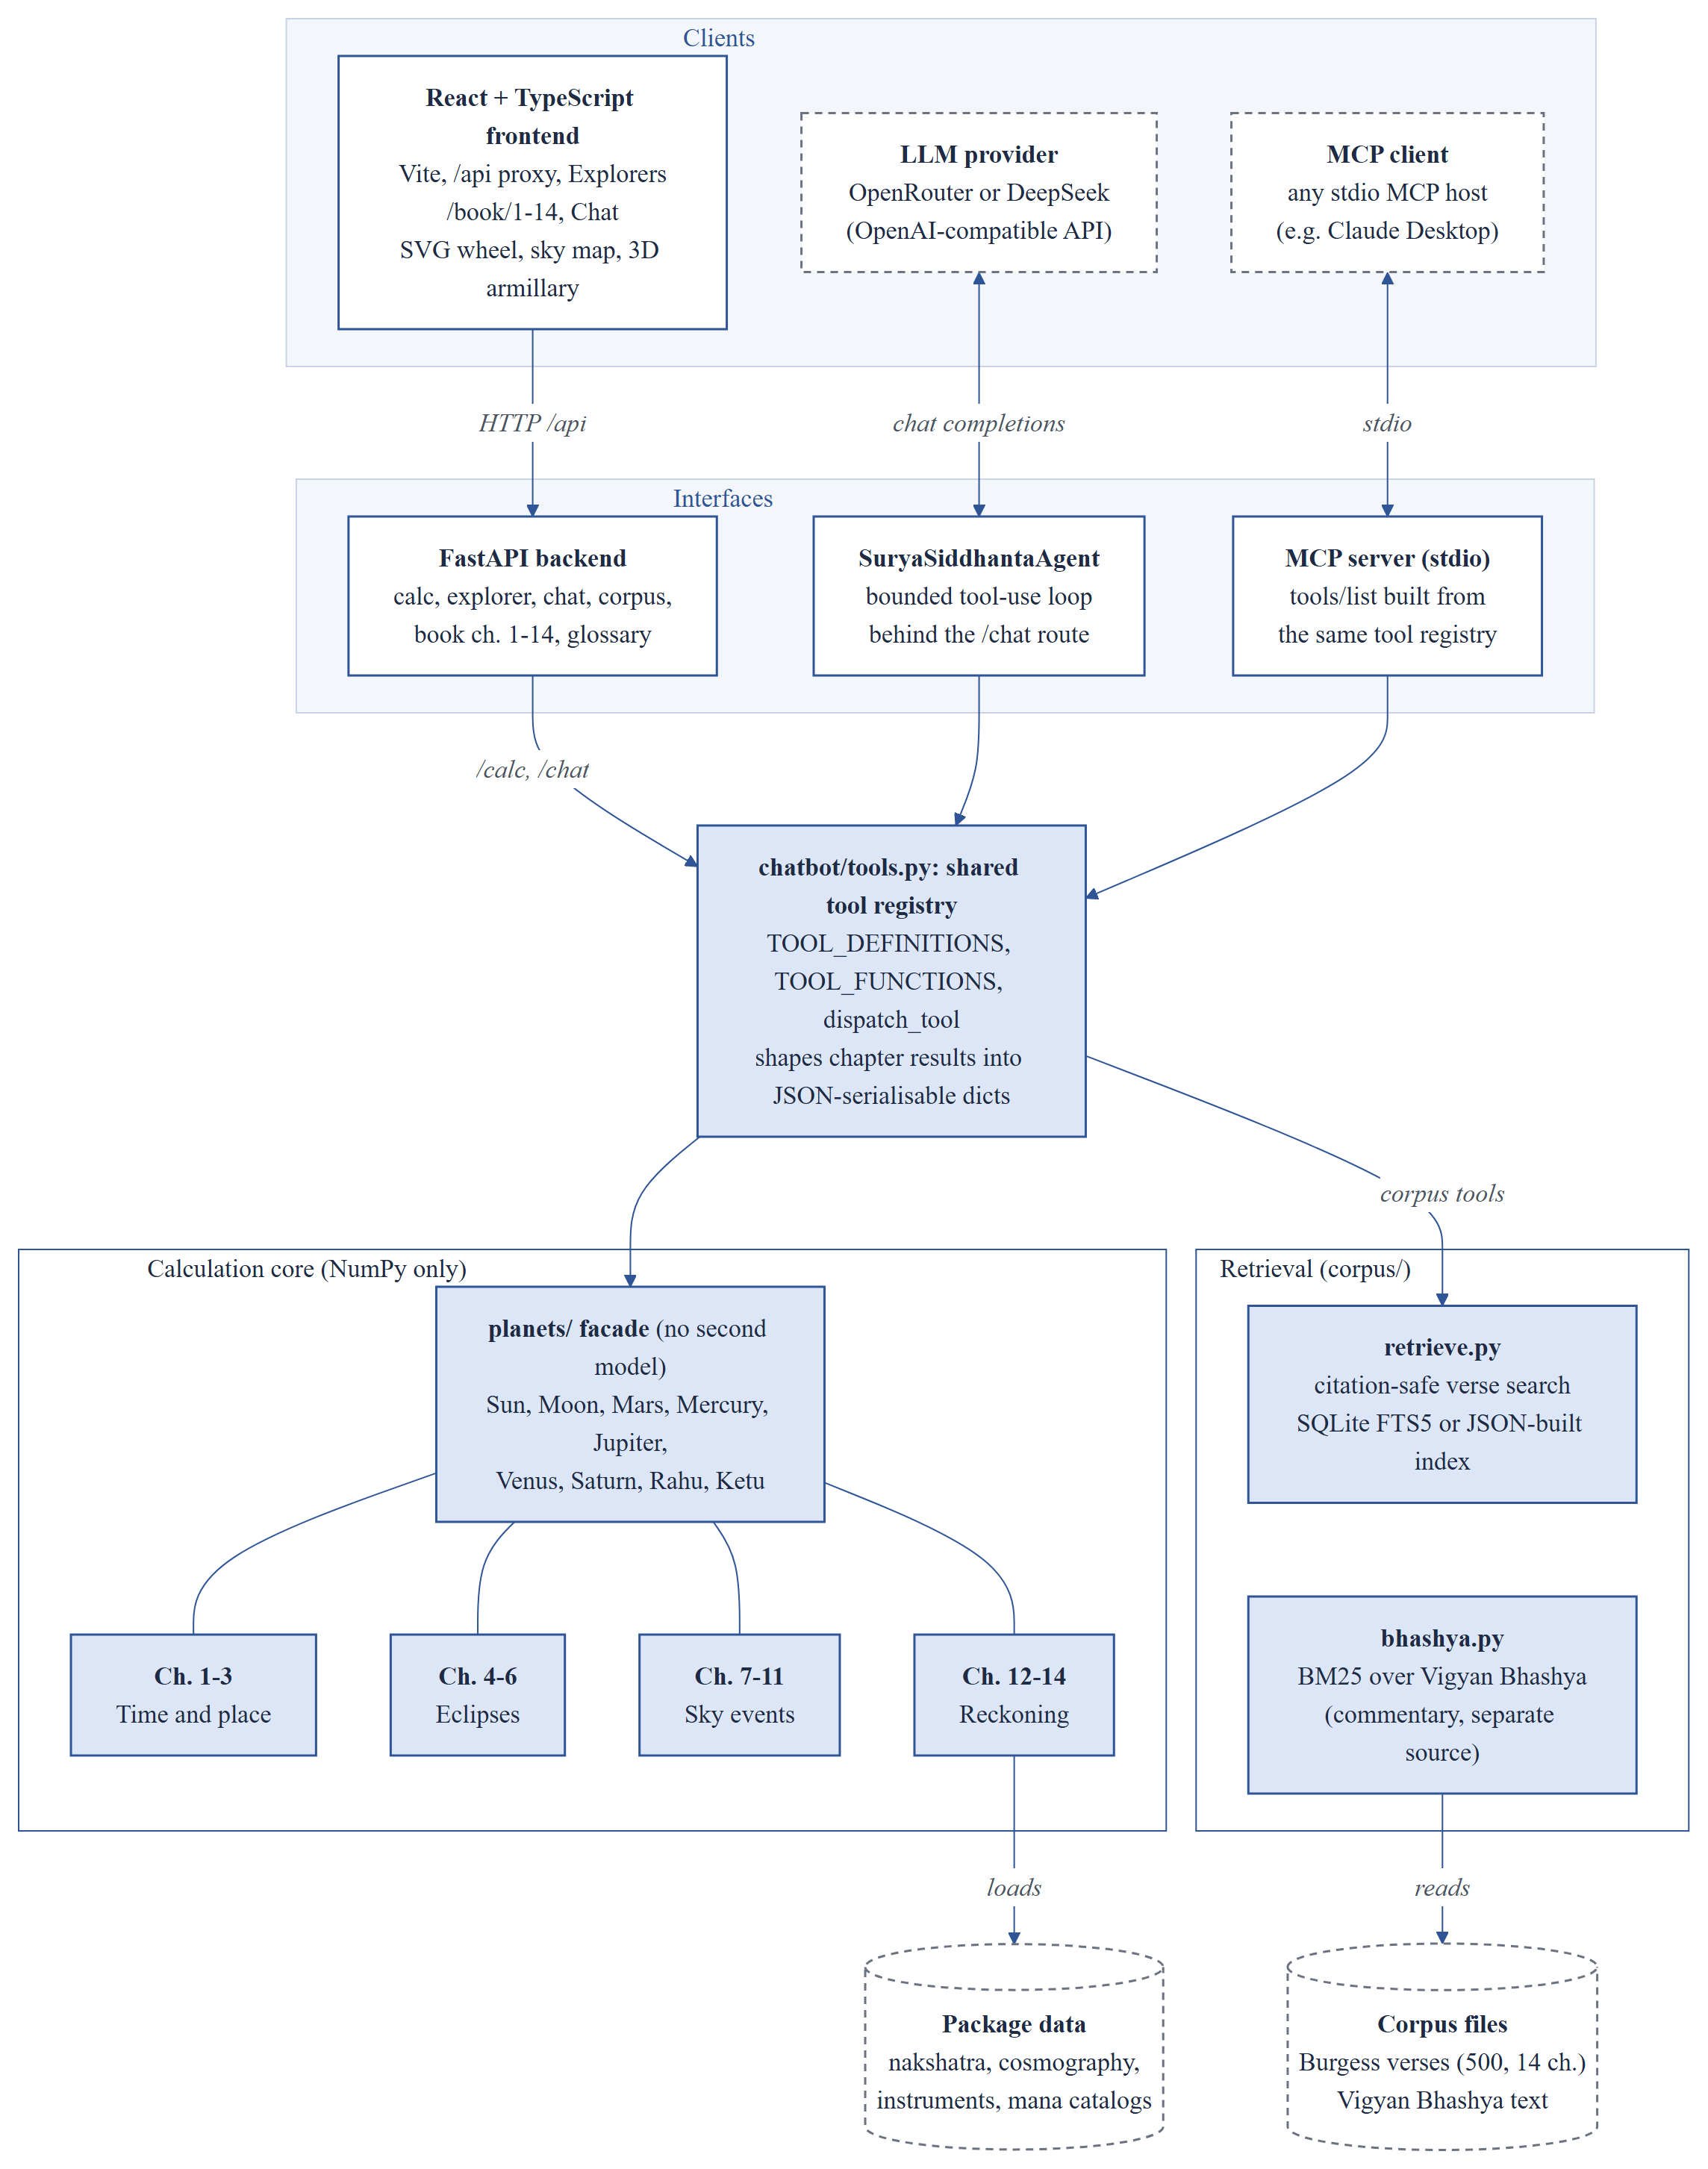
\includegraphics[width=0.85\linewidth,height=0.8\textheight,keepaspectratio]{architecture.png}
  \caption{Layered architecture diagram of the Surya Siddhanta computation library}
  \label{fig:architecture}
\end{figure}

\section{Chapter-wise algorithm implementation}

\subsection{Chapter 1: Mean Motions}

The first chapter of the \emph{\surya} explains the measurement of time, the calculation of elapsed days (\emph{ahargaṇa}) and the mean revolutions of celestial bodies over a \emph{mahāyuga}~\cite{burgess1860}. These calculations form the basis for determining the mean positions of the Sun, Moon and planets. In our implementation, we convert calendar dates into Julian Day, calculate the elapsed-day count and use the revolution constants given in the text to determine the mean longitude of each celestial body. We also calculate the calendar values required for \emph{pañcāṅga} calculations and other chapters. The revolution constants are important because even a small difference in the mean motion can produce a noticeable difference in planetary positions over a long period.

An important part of this chapter is understanding the revolution counts given for Mercury and Venus. Their listed revolutions represent the motion of their \emph{śīghroccas}, while their mean planetary longitudes follow the mean Sun. In our implementation, we treat these quantities separately so that the \emph{śīghra} corrections can be calculated correctly in the later chapters. We also check the calculated positions of Mercury and Venus against their expected limited angular separation from the Sun to identify possible errors in the calculation. For the remaining celestial bodies, we use their respective revolution constants to calculate their mean longitudes. Since mean longitude is a cyclic quantity, we reduce the calculated angular values to the range of 0° to 360°. We maintain separate revolution constants for the seven classical celestial bodies, the lunar node and the lunar apogee. We also consider the retrograde motion of the lunar node by following the appropriate sign convention. In our evaluation, we compare the mean motion rates obtained from the historical revolution constants with modern reference values to understand how differences can accumulate~\cite{Park2021DE440} over long periods. However, we use only the historical constants for calculating the mean positions.

We also consider the epoch as an important part of the calculation because it determines the starting point for the mean motions. The elapsed-day count calculated in Chapter 1 is used in the mean longitude calculations of all celestial bodies. Even an error of one day can change their calculated positions, with different effects on the Moon, Sun and planets because of their different rates of motion. To check these calculations, we implemented date-conversion functions and tests for the epoch, elapsed days and calendar values. During the implementation, we also identified an issue related to the conversion between local time and the historical time reference. This showed that a correct elapsed-day count can still produce incorrect results if the time is interpreted using a different reference meridian. We therefore corrected the time conversion and checked its consistency with the observer's longitude. These calculations and tests provide the time and mean-position values required for the astronomical calculations in the following chapters.

\subsection{Chapter 2: True Positions}

The second chapter of the \surya explains the methods used to calculate the true positions of celestial bodies from their mean positions. It provides a table of 24 jyā (sine) values with a radius of 3438~\cite{burgess1860,plofker2009} and describes the manda and śīghra corrections used in planetary calculations. The jyā values are given at intervals of 225 arcminutes (3°45′). In our implementation, we use interpolation to calculate sine values between the tabulated entries. We then apply the \emph{manda} and \emph{śīghra} corrections in the sequence described in the text, including the required half and full correction stages~\cite{burgess1860,duke2005}. We also follow the sign convention given for the \emph{manda} anomaly, since changing its sign would reverse the direction of the correction and produce an incorrect planetary longitude.

We use modern inverse trigonometric functions and square-root operations to perform these calculations. Although we follow the mathematical methods described in the \emph{\surya}, our implementation does not reproduce every rounding step used in historical manual calculations. The calculation of true longitude is important because the resulting planetary positions are also used in later calculations involving eclipses, conjunctions and calendar determination. For Mercury, Venus, Mars, Jupiter and Saturn, we also apply the \emph{śīghra} correction using an additional moving reference point. The Sun provides this reference for Mars, Jupiter and Saturn, while Mercury and Venus use their respective moving \emph{śīghrocca} positions. In our true\_longitude\_full function, we apply the corrections one after another rather than treating them as independent fixed corrections. The result of each correction is used in the next stage of the calculation. We compare the final calculated longitudes with modern reference values obtained from the DE440 planetary ephemeris~\cite{Park2021DE440} to evaluate the results of our implementation. These comparisons help us understand the differences between the historical astronomical model and modern planetary calculations.

We also calculate the mean longitudes of the Moon and the lunar nodes using their respective mean motions. In our implementation, Rahu represents the ascending lunar node and its longitude is calculated using retrograde mean motion. We do not apply an additional periodic correction to Rahu because the method followed in our interpretation of the text does not provide one. Therefore, the calculated position of Rahu represents a mean lunar node rather than an observed or osculating position. We calculate Ketu, the descending lunar node, by adding 180° to Rahu's longitude and reducing the result to the range of 0° to 360°. When we compare these values with modern lunar-node positions, we consider that differences may arise from the use of a historical mean-node model, different reference definitions and the numerical methods used in our implementation. This distinction helps us interpret the comparison results without treating every difference as an error in the program.

\subsection{Chapter 3: Direction Place and Time}

In Chapter 3, we implemented calculations that connect the positions of celestial bodies with their observed positions from a particular location. We developed functions to calculate directions, gnomon shadows, rising and setting times and the lagna (ascendant). These calculations use the position of a celestial body along with the observer's latitude, longitude and local time. We found that checking only the celestial longitude is not sufficient for verifying these results. The same Julian Day can give different local sidereal times at different meridians, which changes the orientation of the ecliptic relative to the observer's horizon.

During development, we identified and corrected an error related to the Ujjain time convention. Before this correction, some calculations involving parallax and astronomical instruments could produce internally consistent results while representing an incorrect local sky orientation. We corrected the time conversion to maintain consistency between the historical time reference and the observer's local coordinates. We also used the geometrical relationships between the horizon, celestial equator and ecliptic to understand why planetary longitude alone is insufficient for calculating local rising times or the ascendant.

We implemented the gnomon calculation to determine the relationship between the Sun's altitude and the length of its shadow. The lagna calculation identifies the ascending intersection of the ecliptic with the observer's eastern horizon, while the rising and setting functions calculate when a celestial body crosses the horizon. Although these functions use the same observer-based coordinate system, they calculate different astronomical quantities. We tested the functions using known geometrical relationships and numerical examples from Chapter 3. During our review, we also found that an earlier example in the project guide referred to functions that were no longer available. The current implementation is maintained in ch03\_direction\_place\_time.py. This showed us the importance of keeping the project documentation consistent with changes made to the calculation library.

We also examined how celestial coordinates are converted into directions and positions relative to an observer. While ecliptic longitude identifies a position along the ecliptic, calculating the rising or setting of a celestial body also requires its complete position, the obliquity of the ecliptic, local sidereal time and the observer's latitude. We followed the obliquity convention described in the \surya~\cite{burgess1860} for the historical calculations. We found that mixing different time conventions could change the local sky geometry and affect related calculations, as observed in our solar-eclipse parallax example. Through these checks, we established the importance of specifying the coordinate frame, time convention, observer's location and expected numerical values when testing astronomical calculations.

\subsection{Chapters 4 and 5: Eclipses}

In Chapter 4, we implemented lunar-eclipse calculations using the positions of the Sun and Moon along with the geometry of Earth's shadow. In Chapter 5, we implemented solar-eclipse calculations that also require corrections based on the observer's geographical location. Since the Moon's apparent position changes with the observer's location, we included the solar parallax corrections known as lambana and nati. We kept the geocentric calculations separate from the location-specific calculations to make the procedures easier to understand and verify. We also included the observer's location and the date and time conventions in the results because eclipse circumstances can differ between locations. During implementation, we identified some limitations in the eclipse calculation procedures. Our current implementation does not include the complete three-pass asakṛt iteration described in a worked example from Srivastava's commentary~\cite{shrivastava}. Some apparent disc-diameter calculations also use fixed mean values instead of applying all the corrections described in the text. These limitations can affect the calculated beginning and ending times of eclipses. Therefore, we use these modules to demonstrate and examine the implemented historical procedures rather than claiming that they provide fully validated eclipse timing predictions. We used several astronomical quantities in the eclipse calculations, including the difference between the Sun's and Moon's longitudes, the position of the lunar node, apparent disc diameters and local parallax corrections for solar eclipses. We found that differences in these quantities can change the calculated contact times or whether an eclipse is predicted for a particular location. We maintained separate modules for lunar and solar eclipses because they involve different geometrical conditions. Lunar-eclipse calculations use the relationship between the Moon and Earth's shadow, while solar-eclipse calculations also consider the Moon's apparent position from the observer's location. We compared intermediate values, including lambana and nati, with the worked numerical examples provided in the commentary~\cite{shrivastava}. These comparisons helped us identify implementation errors, although agreement with individual examples does not establish the accuracy of all eclipse predictions.

We also made the lunar- and solar-eclipse calculations accessible through the project's API routes and user interfaces. For solar eclipses, users can provide their geographical latitude and longitude to calculate location-dependent results. We kept the evaluation of planetary longitudes separate from the evaluation of eclipse events. Our DE440~\cite{Park2021DE440} comparison study measures longitude differences over a long period using samples taken at ten-day intervals, but it does not directly evaluate eclipse contact times. We therefore do not use those longitude comparisons as evidence of minute-level accuracy in eclipse predictions. A separate evaluation using observed or independently calculated eclipse events would be required to assess the accuracy of the predicted contact times.

\subsection{Chapter 6: Eclipse Projection}

In this chapter, we implemented functions to represent eclipse calculations through diagrams showing the contact points, apparent discs and relative positions of celestial bodies. We kept the diagram generation separate from the eclipse calculations so that the numerical results could be verified independently before plotting. The diagrams help users understand the geometrical relationships involved in an eclipse. We also made plotting optional so that users who only need numerical results can use the calculation library without requiring additional graphics dependencies.We designed the eclipse diagrams to display the relevant lines, apparent discs, contact points, date and observer's location. The diagrams also distinguish between results obtained from the historical \emph{\surya} model and those obtained from modern reference data, where applicable. We used the angular values calculated in the earlier chapters to construct these diagrams. The visual representations are intended to explain the calculated geometry and should be interpreted according to the assumptions and coordinate conventions used in the eclipse calculations.

We also used these diagrams to examine the relative positions and paths of the celestial bodies during an eclipse. The contact points, apparent discs and shadow paths help explain the results to users who may not be familiar with traditional astronomical terminology. They can also help identify errors such as reversed directions or incorrectly positioned shadows that may not be immediately visible from numerical values alone. We kept the numerical diagram data separate from the plotting code so that the calculations can be tested without requiring a graphics system. We also provided support for generating diagrams using Matplotlib~\cite{hunter2007} when a visual representation is required.We used the diagrams as an additional way to check the consistency of eclipse calculations. For example, the direction of the relative path should agree with the signs of the calculated latitude and contact offsets under the selected coordinate convention. If the diagram shows an incorrect direction, we can examine whether the problem comes from the coordinate conversion, plotting procedure or underlying event calculation. By keeping the numerical geometry separate from the optional plotting functions, we made it easier to test these components independently. The generated figures can also be presented alongside tables of the corresponding contact values, allowing readers to compare the numerical results with their visual representations.

\subsection{Chapters 7 and 8: Conjunctions and Stars}

In Chapter 7, we implemented functions to find conjunctions between planets and between planets and junction stars. Chapter 8 provides information about stars and \emph{nakṣatras}, including their names and coordinates. We developed functions to identify a \emph{nakṣatra} from a given longitude and calculate the rising and setting of stars. Since conjunctions depend on the changing positions of celestial bodies, we implemented a search across a range of dates rather than calculating conjunctions from a single date. We used the star catalogue to obtain the names and coordinates required for these calculations.

We found that the coordinates of junction stars can be interpreted in different ways. In Chapter 8, we used an ecliptic interpretation of the star catalogue, while Chapter 13 follows a polar-coordinate method for placing stellar hoops on the armillary sphere. These two methods produce different declination values for some stars. We kept both interpretations in our implementation rather than applying a single coordinate method to all calculations. This allows us to preserve the differences between the procedures described in the two chapters.

We also implemented the \emph{nakṣatra} lookup using the divisions of the ecliptic circle into asterisms and their smaller portions. For fixed-star calculations, we used the coordinates stored in the star catalogue. In our computational-edition study, we calculated~\cite{nigam2026edition} the listed \emph{dhruvaka} values using the shares given in the verses and examined the effect of rounding on the catalogue values. We found that Chapter 13 uses a different procedure for constructing stellar hoops. By comparing the results of both methods for a selected star and date, we can observe how their calculated positions differ. However, this comparison alone does not establish which interpretation is historically correct.

We organised the star data in the nakshatra\_catalog.json file and connected it with the corresponding calculation functions. This allows users to examine a star's reference verse in the corpus browser while using its coordinates in astronomical calculations. In our computational-edition study, we found~\cite{nigam2026edition} that the \emph{dhruvaka} values for twenty-seven stars follow a rule based on each star's assigned share and the accumulated minutes of the preceding asterisms. We also observed a small difference in the stored value for Revatī due to rounding in the catalogue. This example shows why we need to consider the precision of historical values when comparing them with calculated results and their numerical representation in the software.

\subsection{Chapters 9 and 10: Visibility and The Moon}

In Chapter 9, we implemented functions to calculate the heliacal rising and setting of planets and stars. These events occur when a celestial body becomes visible again after being hidden by the Sun's brightness or disappears from visibility near the Sun. Since heliacal events are different from geometrical conjunctions, we developed separate functions to search for the next rising or setting event. In Chapter 10, we implemented calculations for the Moon's elongation, illuminated fraction, phase, crescent width, horn angle, moonrise and moonset. Some of these calculations use the positions of the Sun and Moon, while others also require the observer's geographical location. We used the astronomical position calculations from earlier chapters to calculate these additional quantities. For example, we estimated the Moon's phase using its angular separation from the Sun, while moonrise and moonset calculations also require the observer's location. We also considered that naked-eye visibility cannot be determined from geometrical positions alone. Therefore, we kept the visibility calculations separate and documented the specific rules used to estimate heliacal events.

In Chapter 10, we used the Sun--Moon geometry to calculate several lunar properties. The elongation represents the angular separation between the Sun and Moon, while the illuminated fraction describes the visible portion of the lunar disc. We used additional geometrical relationships to calculate the crescent width and horn angle. For moonrise and moonset, we included the observer's geographical location in the calculations. We also provided a complete example of the Chapter 10 functions in the project guide and added tests to verify their results. For heliacal events, we implemented a forward search from a given Julian Day to identify the next event without requiring users to provide its date. The results are presented with the visibility rule used in the calculation so that users can understand the assumptions behind them.

We also developed different visual interfaces to present these calculations. The positions page displays the Sun and Moon on a zodiac wheel, while the Moon page shows the lunar phase and crescent shape. The star page provides a sky map to help users understand the positions of celestial bodies. These interfaces also show why different calculations require different input information. For example, the Moon's phase can be estimated using a date, whereas moonrise and moonset also require a location. When location and UTC offset information is available, we pass it to the chatbot as part of its context. We also designed the chatbot tools to identify the location and time convention used when presenting calculation results.

\subsection{Chapter 11: Patas}

In Chapter 11, we implemented the calculations for Vyatipāta and Vaidhṛta, which are \emph{pāta} events associated with the declinations of the Sun and Moon. We calculated these events by applying the Moon's latitude correction to its declination and searching for the instant when the required declination condition is satisfied. We also calculated the beginning and ending times of each event using the relevant daily motions. These \emph{pāta} events are different from the daily pañcāṅga \emph{nitya-yoga} categories, although they share the same names. We maintained this distinction in the implementation to avoid confusion between the two calculation methods. During verification, we identified an error in the calculation of the \emph{pāta} event duration. Our earlier implementation used the rate at which the calculated solar and lunar declinations separate. However, after checking the relevant verse, we found that the denominator should use the difference in daily motions specified in the text. We corrected this calculation because the choice of denominator affects the beginning and ending times of the event, even when the calculated central instant remains reasonable. This example helped us understand the importance of following the specific mathematical procedure given in the source rather than using a different method that appears geometrically suitable.

We made the Chapter 11 calculations available through the find\_patas and compute\_pata\_details chatbot tools, REST API endpoints and the Patas page. These interfaces allow users to find \emph{pāta} events and examine their calculated details. We also added tests to check that the event calculations follow the documented interpretation. The central instant is determined using the declination condition, while the event duration is calculated separately using the motion values specified in the verse. We kept these calculations separate so that an error in the duration formula can be identified without affecting the verification of the central event instant.

We also documented the correction in the implementation changelog and maintained the distinction between \emph{pāta} events and the daily pañcāṅga \emph{nitya-yoga}. The latter is calculated using the sum of the Sun's and Moon's longitudes and represents a different calendrical quantity. Through this implementation, we found that even a small difference in the interpretation of a mathematical rule can change the calculated duration of an astronomical event. By checking the central declination condition and the duration calculation separately, we made the results easier to verify and review.

\subsection{Chapter 12: Cosmography}

In Chapter 12, we implemented calculations related to the Earth's globe, planetary orbit distances and different cycles of time described in the \surya. We calculated the planetary orbit distances using the Moon's stated distance of 324,000 yojanas and the assumption that all celestial bodies travel the same total linear distance during a yuga. We also implemented functions to calculate the Earth's circumference, the circumference adjusted for geographical latitude and the longitude difference correction used in other chapters. These calculations follow the historical mathematical model of the \surya and should not be treated as modern measurements of astronomical distances.

We also found that Chapter 12 contains several descriptive concepts that cannot be directly converted into numerical calculations. These include the order of creation, divisions of cosmic time and other cosmological descriptions. To preserve this information, we developed a verse-tagged data catalogue that stores the descriptive content along with its source references. This allows our web interface to present both numerical results and explanatory material without treating every statement in the chapter as a measurable astronomical quantity.

For the planetary orbit calculations, we used the common linear-distance rule along with the revolution counts given in Chapter 1. We compared the calculated orbit values with those stated in the text and found that they agreed within approximately 1.3 yojanas, as recorded in our project changelog~\cite{nigam_repo}. The small differences are mainly associated with arithmetic and rounding in the historical calculations. We also found that the calculated solar orbit is consistent with a constant used in our lunar-eclipse module. This provided an internal consistency check between different chapters of our implementation. However, these results only demonstrate agreement within the historical mathematical model and do not establish the physical accuracy of the distances when compared with modern astronomical measurements.

We organised the numerical and descriptive parts of Chapter 12 separately within the module. The numerical functions cover Earth dimensions, planetary orbit calculations and time regents, while the data catalogue stores descriptive cosmological information linked to the corresponding verses. This approach allows users to explore the mathematical procedures and read the related explanations through the same application. Through this chapter, we demonstrated how computational and descriptive material from the \surya can be represented together in software while keeping their different purposes clear.

\subsection{Chapter 13: Instruments}

This Chapter mainly discusses astronomical instruments along with some planetary and time-related calculations. In this project, the gola-yantra is implemented as a parametric armillary sphere using an equatorial coordinate frame. Different hoops representing the equator, ecliptic, horizon, colures, solar paths, and stars are generated by the computational module and then passed to the renderer. The React interface provides an interactive three-dimensional view of this model~\cite{react,threejs}, while the actual astronomical geometry is kept separate from the graphics library.

The chapter also includes the implementation of the clepsydra and different methods of finding time using the gnomon, wheel, arc, and staff. Some of these procedures are not described completely in the original verses, so Burgess's commentary is used where additional steps are required~\cite{burgess1860}. To make this clear, every calculated output identifies its source category. This helps the user understand whether a calculation is directly supported by the verses or is based on a reconstruction using commentary to complete an incomplete description.

In the armillary model, each hoop is stored using its geometric plane and offset. This allows the renderer to construct the complete sphere without performing the astronomical calculations again. Some parts of the model change depending on the observer's location and time. For example, the orientation of the horizon and the position where the ecliptic crosses the horizon depend on local conditions, while some reference circles remain fixed in the equatorial frame. The interactive interface makes these changes easier to understand visually. This chapter also shows why source labelling is important in the project. In some cases, a verse mentions an instrument but does not provide every mathematical step required to calculate time using it. In such cases, the implementation may use the procedure explained in Burgess's commentary. The software clearly mentions when such an additional rule has been used instead of presenting the reconstructed procedure as if it came directly from the original verse. This makes the source and limitations of the calculation more transparent.

The Chapter 13 implementation uses an equatorial coordinate system in which the north-pole direction and equinox axes are fixed by convention. Each hoop is treated as a geometric object inside this coordinate frame. The renderer can rotate or change the visual viewpoint without changing the astronomical values stored by the computational model. For Ujjain, the computational-edition manuscript reports that the armillary model contains 46 hoops~\cite{nigam2026edition}.

The implementation also calculates the point where the ecliptic intersects the eastern horizon directly rather than estimating it by interpolation between zodiac signs. Using interpolation could make the movement in the three-dimensional visualization appear smooth, but it could also produce an inaccurate local ascendant. Therefore, the project calculates this point directly from the geometry. This separation between astronomical computation and visual rendering helps maintain the accuracy of the model while still allowing an interactive three-dimensional representation.

\subsection{Chapter 14: Reckoning of Time}

In this chapter, we implemented the calendar and time-related calculations described in the \surya. These include different measures of time, solar ingress, months, seasons and named Jovian years. We used the solar-position calculations from earlier chapters along with the historical day count to maintain consistent date and meridian conventions throughout the implementation.

We also implemented two methods for identifying the Jovian year. The first method follows the original verses, while the second uses the mean-longitude method described in Burgess's commentary~\cite{burgess1860}. We kept these methods separate so that users can identify which source was followed for each result.

We developed a catalogue of mānas to convert between different traditional units of time. The module also calculates solar ingress events for a given Gregorian year, ayanas, equinox crossings, ṣaḍaśītimukha divisions, the Fathers' day and Jupiter's named-year cycle. We provided the barhaspatya\_year function with an option to select the calculation method. The output includes the calculated Jovian year name along with the method used to obtain it.

We implemented the solar\_year function using the Sun's entry into Aries as the beginning of the solar year. Related functions calculate seasonal divisions and other solar ingress events. We also developed the pitrya\_clock function to calculate the Fathers' day using the relationship between the Sun and Moon. We kept these calculations as separate functions because they represent different calendrical procedures rather than a single general calendar conversion method.

\section{Public interfaces}

The project includes multiple user interfaces built around the same computational library. The earlier Gradio and Streamlit applications~\cite{gradio,streamlit} provide features such as planetary positions, panchanga, eclipses, and other calculations. The current React application uses FastAPI~\cite{react,fastapi} for calculations, chapter browsing, corpus search, glossary access, and chat. Although the interfaces are different, they all use the same chapter-level calculation functions.

Using one common calculation layer helps keep the results consistent across interfaces. However, input conversion, formatting, and API response handling tested using test cases. All the validation here comes from source comparisons, worked examples, and tests.

The React interface also includes pages for Cosmography, Instruments, chapter and verse browsing, learning paths, and research views. SVG and 3D components are used to explain geometric concepts like universe explorer. The REST API returns structured results so that other applications can also reuse the same calculations.

Users can read verses, run calculations, inspect related geometry, and use glossary entries to understand technical terms. The learning paths reuse the Chapter 1 and 2 APIs, while the Research Explorer displays saved evaluation results. The source code and tests provide the final record of how each calculation is implemented.

\subsection{Technologies used}
\label{sec:technologies}

We have mainly used Python and React. But we have also used different packages on specific part of the project, while the main calculation library still remains independent of the web interface and AI model providers. This table summarizes the technologies used in the current implementation as well as the earlier interfaces developed during the project.

\begin{longtable}[]{@{}
  >{\raggedright\arraybackslash}p{(\linewidth - 2\tabcolsep) * \real{0.2632}}
  >{\raggedright\arraybackslash}p{(\linewidth - 2\tabcolsep) * \real{0.7368}}@{}}
\caption{Technologies and their roles}\label{tab:technologies}\\
\toprule\noalign{}
\textbf{Area} & \textbf{Technologies and role} \\
\midrule\noalign{}
\endfirsthead
\caption[]{Technologies and their roles (continued)}\\
\toprule\noalign{}
\textbf{Area} & \textbf{Technologies and role} \\
\midrule\noalign{}
\endhead
\bottomrule\noalign{}
\endlastfoot
Calculation library & Python and NumPy implement the numerical methods~\cite{python,harris2020}; Matplotlib supports plots and eclipse diagrams~\cite{hunter2007}. \\
Backend and contracts & FastAPI, Pydantic and Uvicorn~\cite{fastapi,pydantic,uvicorn} provide REST endpoints, request validation and the ASGI server. \\
Current web interface & React JS, TypeScript, Vite, React Router~\cite{react,typescript,vite}, HTML and CSS provide the browser application. \\
Geometry and text & Three.js, React Three Fiber and Drei support 3D views~\cite{threejs,r3f}. KaTeX, React Markdown and remark-gfm~\cite{katex} display equations and formatted text. \\
Earlier interfaces & Streamlit and Gradio were used for the earlier~\cite{streamlit,gradio} calculation, panchanga and chatbot interfaces. \\
AI providers and tools & OpenRouter and DeepSeek APIs provide model access through the OpenAI Python SDK~\cite{openrouter,deepseek,openaisdk}. Tool calling and MCP connect models~\cite{mcp} to project functions. \\
Corpus and retrieval & SQLite FTS5 and BM25 support indexed search~\cite{sqlitefts5,robertson2009}. JSON and JSONL hold corpus exports and processing records. \\
OCR and translation & Gemma 4 E2B, Surya OCR 2, Sarvam Document Intelligence and Patram were explored~\cite{gemma,suryaocr,sarvam,patram} for document extraction and translation. \\
Model runtimes & LM Studio and Hugging Face Transformers support local model work~\cite{lmstudio,wolf2020transformers}; the Transformers path uses PyTorch~\cite{paszke2019pytorch}. \\
Document preparation & PyMuPDF, OpenCV and Pillow support PDF extraction~\cite{pymupdf,bradski2000opencv,pillow} and page-image processing. python-docx and Markdown outputs support document export. \\
Checks and delivery & pytest and Playwright support software checks~\cite{pytest,playwright}. Docker and Docker Compose package the services~\cite{merkel2014docker}; Git and GitHub track and share the source. \\
\end{longtable}

\section{Corpus preparation retrieval and chatbot}
\label{sec:corpus-chatbot}

\subsection{Source extraction and corpus construction}

There is a separate ss\_corpus project~\cite{nigam_sscorpus} we created to prepare machine-readable content from the English Burgess edition and the scanned Hindi edition Vigyan Bhashya~\cite{burgess1860,shrivastava}. It used text extraction, OCR, cleaning, and verse segmentation. For the Hindi text, legacy fonts were also checked, and text was converted to Unicode. After that this extracted content was reviewed page by page before being stored as verse records which helped to reduce the error during OCR and translations.

I tested different model based extraction methods which prose Devanagari text, equations, and tables created a different OCR challenges. This table summarizes the models and outputs used in these experiments.

\begin{longtable}[]{@{}
  >{\raggedright\arraybackslash}p{(\linewidth - 2\tabcolsep) * \real{0.2632}}
  >{\raggedright\arraybackslash}p{(\linewidth - 2\tabcolsep) * \real{0.7368}}@{}}
\caption{OCR and translation work}\label{tab:ocr}\\
\toprule\noalign{}
Model or service & Recorded work \\
\midrule\noalign{}
\endfirsthead
\caption[]{OCR and translation work (continued)}\\
\toprule\noalign{}
Model or service & Recorded work \\
\midrule\noalign{}
\endhead
\bottomrule\noalign{}
\endlastfoot
Gemma 4 E2B~\cite{gemma} & The saved gemma4\_v2 pass records Hindi OCR and page-level English translation for all 838 scanned pages. \\
Surya OCR 2~\cite{suryaocr} & The saved run records OCR for all 838 pages, with page Markdown and Word exports. \\
Sarvam Document Intelligence~\cite{sarvam} & Notebook runs produced combined Hindi HTML, Markdown, text and a reflowed PDF. \\
Patram~\cite{patram} & Notebook experiments explored transcription and translation of scanned Indic document pages. \\
\end{longtable}

The gemma4\_v2 progress record shows that all 838 pages were completed for OCR and page-level English translation. The Surya OCR record also shows 838 completed pages. Page caches, progress logs, and combined output files help the process continue from where it stopped without repeating already completed pages. However, this completion only means that every page was processed. It does not mean that each word, formula, or translation was checked manually. We have created a 28 page randomly selected document typed by human. Then these results were compared against this document to verify the correctness.

We also used models For the English verse corpus, the pipeline cleans the OCR text, identifies chapter and verse boundaries, separates verse translation from commentary, adds topic information, and connects relevant passages with calculation tools. Each record had a stable verse ID, chapter and verse numbers, language information, and source metadata. These records are stored in JSON and JSONL formats, we also used SQLite FTS5 for indexed search with BM25 ranking~\cite{sqlitefts5,robertson2009}.

The application uses a corrected Burgess corpus containing 500 numbered English verses from all fourteen chapters~\cite{nigam_corpusaudit}. We have used the multi-model steps, which help us to correct the missing verses and incorrect verse commentaries. An earlier ss\_corpus export contains 455 records, so it is different from the corrected version used in the application. The current bundled records do not contain populated Hindi translation fields. The Hindi OCR and English translations of the Hindi book are still separate outputs and are not yet combined as a verse-aligned bilingual corpus.

The corpus is mainly used for chapter browsing, verse search, and source retrieval. It does not provide modern planetary positions for the calculations, because those are still handled by the chapter functions. Having complete numbered-verse coverage also does not mean that the transcription is completely error-free or that the corpus is a complete critical edition.

\subsection{Retrieval and AI Query Interface}

We have also developed the AI chatbot Query Interface. this Interface combines calculation tools with chapter and verse-based text retrieval. We have instructed it to use the chapter-wise corpus core library for all the calculations. It is also implementing a rag-based text retrieval~\cite{lewis2020rag}, which is helping it to explain the quotes in the text. Before explaining or quoting the text, it retrieves the relevant passage along with its verse ID and source information. The retrieval system can use either a SQLite database or an FTS5 index created from the bundled JSON corpus~\cite{sqlitefts5}.

We implemented in a way that, by default the chatbot, corpus search, and Verse Explorer use the all verses from Burgess book export. It can also use the other JSON and database sources if it requires. The Burgess's translated verses and Srivastava's Vigyan Bhashya are kept as separate sources~\cite{burgess1860,shrivastava}. Numerical results come from the calculation functions, while the text retrieval is used for explanation and citation.

This assistant can connect to OpenRouter, DeepSeek, or another compatible model endpoint using the OpenAI Python SDK~\cite{openrouter,deepseek,openaisdk}. This is written in a way that The MCP exposes the same calculation and retrieval tools~\cite{mcp} through standard input and output, while the connected client provides its own model. The retrieval system supports verse lookup, chapter ranges, search, and chapter indexing. If a SQLite index is missing or empty, the application can build a search index from the bundled corpus. This allows the chatbot to search and cite the Burgess text without depending on the external OCR pipeline. However, the quality of the final explanation still depends on the retrieved passage, commentary coverage, and transcription accuracy.

\section{Test strategy}

We used three levels of verification. The Verse-based tests check whether each function follows the selected textual rule or not. The worked examples were checked whether a sequence of calculations reproduces the values printed in the source. The DE440~\cite{Park2021DE440} comparison measures how much a selected longitude calculation differs from a modern astronomical reference. All these methods check different types of errors, so no single test is enough by itself.

The computational-edition manuscript reports 1,256 chapter~\cite{nigam2026edition} and per-planet interface tests and 257 selected worked-example cases.

For the tests We followed the structure of Chapters 1-14, with additional tests for other application components. A recent DE440~\cite{Park2021DE440} revalidation also used a focused Chapter 1-2 suite~\cite{nigam2026de440} of 263 tests. These figures belong to different test runs and should not be combined into a single total.

\section{Web Application, Learning and research interfaces}
\label{sec:learning-interfaces}

The React\cite{react} and FastAPI \cite{fastapi} application is deployed at
\url{https://surya-siddhanta-latest.onrender.com/}. This section
describes each menu and pages under it. Every number on these
pages comes from the chapter modules through the FastAPI routes. The
front-end draws and tabulates results but has no astronomy of its own.

\subsection{Layout and common controls}

The window has three parts. A sidebar on the left side which holds the menus. The
centre shows the selected page. The side panel on the right side holds the AI
assistant and the glossary (Terms) and it can be opened or closed at any time.
Opening the site lands on Planet Positions Page by default. The sidebar groups its
links under five headings: Learn, Explorer, Almanac, AI and The Book.
On the Universe Explorer the sidebar collapses on small screen into an
``All tools'' menu button.

Most pages share the same inputs. The date input has year, month and
day fields. Where the time of day matters, a time-zone field (hours
from UTC, IST by default) is added and the day may be entered with a
fraction for the time of day. The Panchanga page shows the clock time
in its own field. The Pages that depend on the observer adds latitude and
longitude fields, which start at Ujjain. Most pages recomputes as soon
as an input changes, the pages that search over a period (Conjunctions,
Heliacal Events and Patas) have a Search button instead. A three-way switch at the top right of the
content area selects the Light, Dark or Auto theme, which Auto follows the
browser's setting. The footer names the author, roll number and
institute, and states the source of the calculations on the current
page. Its ``About this project'' link opens a dialog with the project
title and links to the source repository, this report, the
presentation, the two papers, the PyPI package and the Docker image.
The dialog also opens by itself on a user's first visit
(Figure~\ref{fig:ui-about}). A round button at the bottom right opens
the AI and glossary panel from any page. Figure~\ref{fig:ui-layout}
shows the layout with the Planet Positions page open. The screenshots
in this section were taken from the deployed site on 24 November 2026
with the default inputs (that date, Ujjain, IST).

Table~\ref{tab:ui-menus} lists every page with its inputs and its main
outputs.

\begin{figure}[htbp]
  \centering
  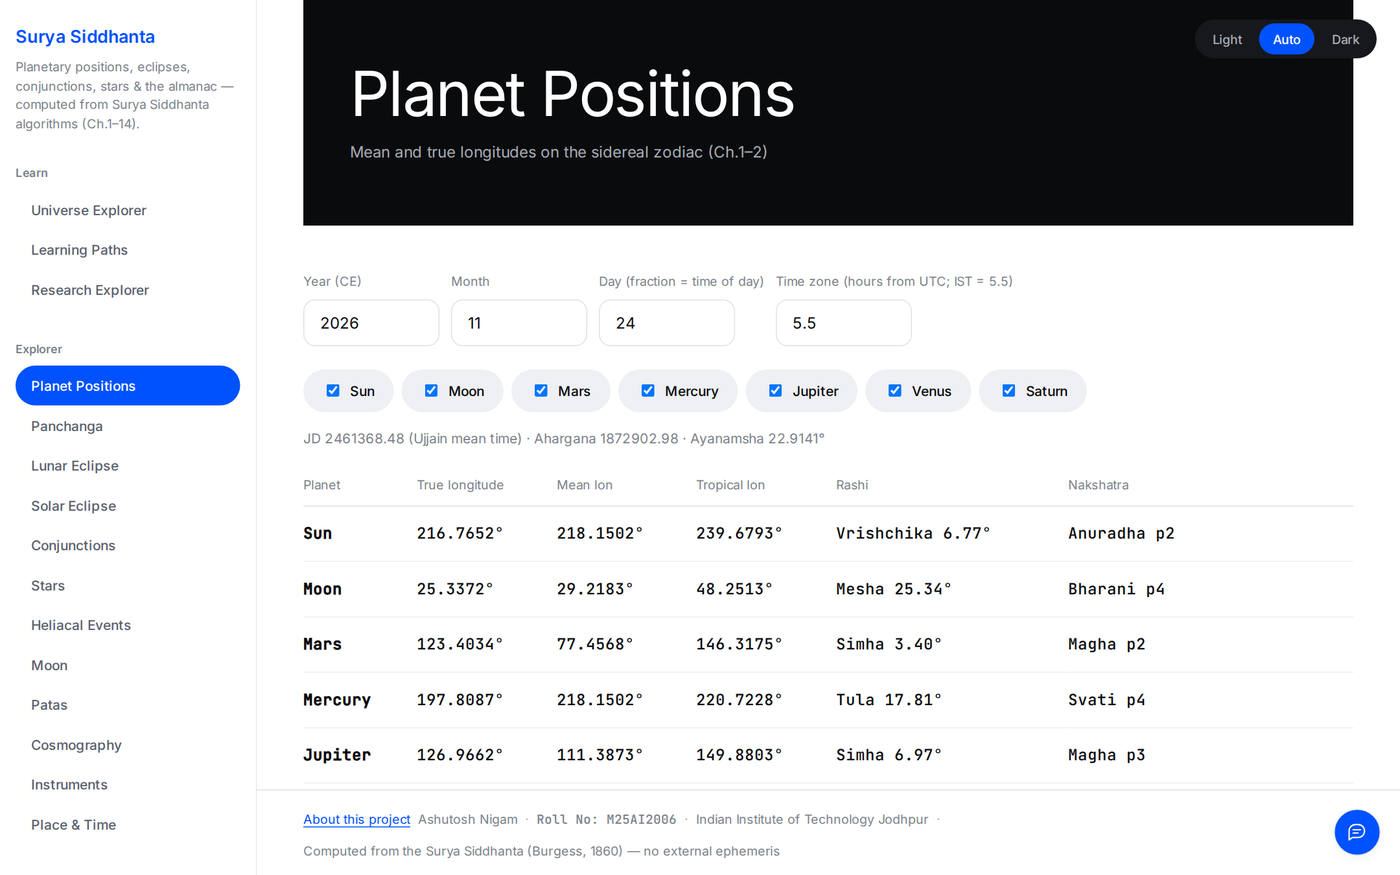
\includegraphics[width=\linewidth,height=0.62\textheight,keepaspectratio]{ui/ui-layout.png}
  \caption{Application layout: sidebar menus on the left and the Planet Positions page in the centre}
  \label{fig:ui-layout}
\end{figure}

\begin{figure}[htbp]
  \centering
  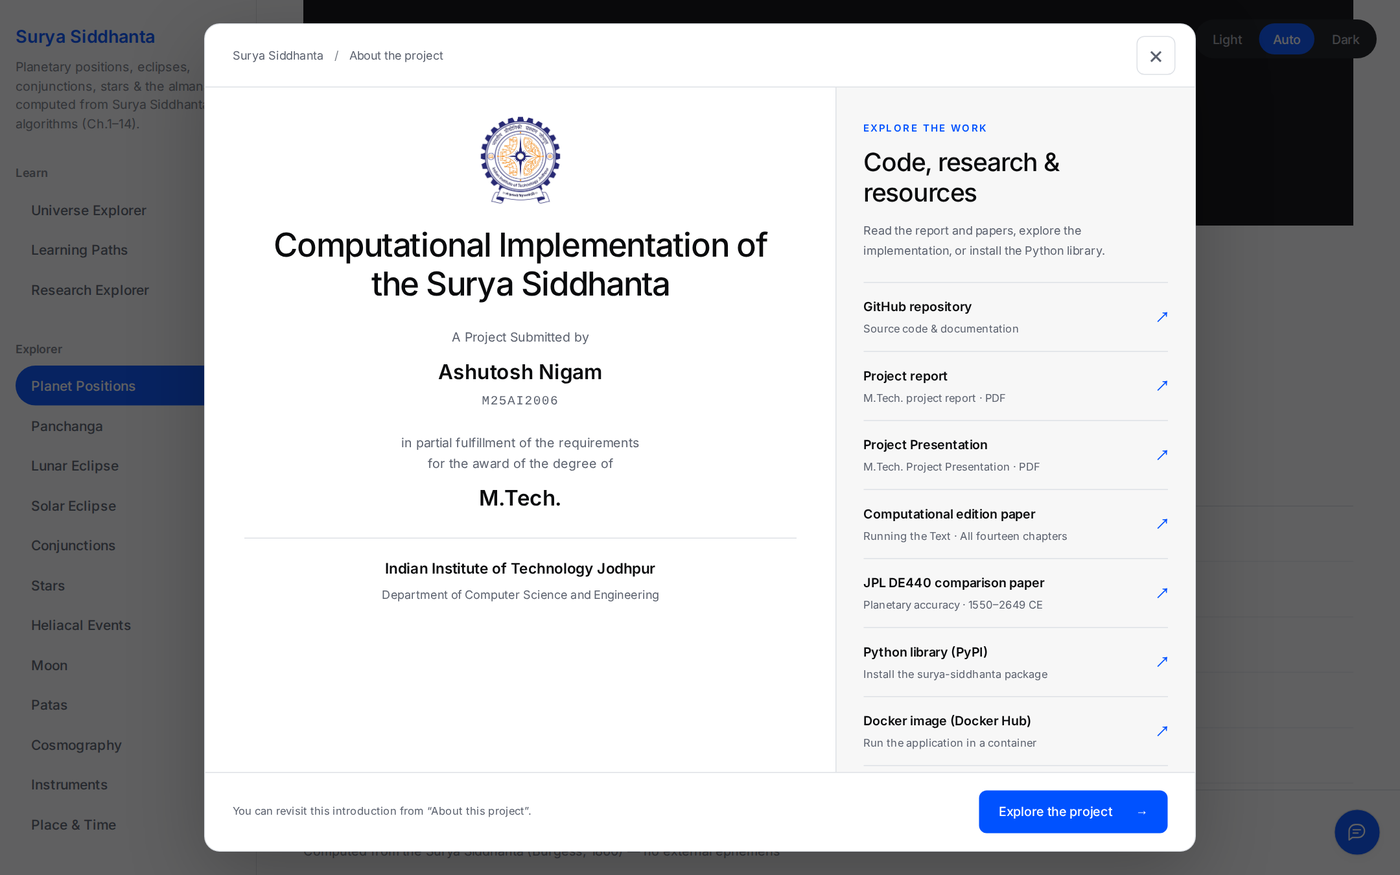
\includegraphics[width=\linewidth,height=0.62\textheight,keepaspectratio]{ui/ui-about.png}
  \caption{The ``About this project'' dialog with links to the code, papers and packages}
  \label{fig:ui-about}
\end{figure}

\begin{longtable}[]{@{}
  >{\raggedright\arraybackslash}p{(\linewidth - 6\tabcolsep) * \real{0.1500}}
  >{\raggedright\arraybackslash}p{(\linewidth - 6\tabcolsep) * \real{0.2000}}
  >{\raggedright\arraybackslash}p{(\linewidth - 6\tabcolsep) * \real{0.2800}}
  >{\raggedright\arraybackslash}p{(\linewidth - 6\tabcolsep) * \real{0.3700}}@{}}
\caption{Menus and pages of the web application}\label{tab:ui-menus}\\
\toprule\noalign{}
\textbf{Menu} & \textbf{Page} & \textbf{Inputs} & \textbf{Main outputs} \\
\midrule\noalign{}
\endfirsthead
\caption[]{Menus and pages of the web application (continued)}\\
\toprule\noalign{}
\textbf{Menu} & \textbf{Page} & \textbf{Inputs} & \textbf{Main outputs} \\
\midrule\noalign{}
\endhead
\bottomrule\noalign{}
\endlastfoot
Learn & Universe Explorer & Model, body, time and play speed & 3D or 2D
view of the bodies, planet details, guided tours, ``Ask Surya''
chat \\
Learn & Learning Paths & Lesson date and correction stage & Eight
lessons (Sun to Saturn and Rahu) with diagrams, checks and JSON
export \\
Learn & Research Explorer & Body and 100-year window & Saved DE440 RMS
matrix, residual chart, JSON and CSV downloads \\
Explorer & Planet Positions & Date, time zone, planet checkboxes & Mean,
true and tropical longitude, rashi, nakshatra and pada, zodiac
wheel \\
Explorer & Panchanga & Date, clock time, time zone & Tithi, vara,
nakshatra, yoga, karana, masa, ritu, samvatsara, Sun and Moon
longitude, ayanamsha \\
Explorer & Lunar Eclipse & Date near full moon & Eclipse type,
magnitude, Moon latitude, Moon and shadow diameters, half-duration,
totality \\
Explorer & Solar Eclipse & Date near new moon, latitude, longitude &
Eclipse type, magnitude, disc diameters, lambana and nati parallax,
half-duration, Sun's altitude, local visibility \\
Explorer & Conjunctions & Two planets, start year, span in months (up
to 60) & Date, longitude, separation and type of each conjunction \\
Explorer & Stars & Date, time zone, nakshatra & Junction star, deity
and gana, span, sidereal, tropical and equatorial position, rise and
set, sky map \\
Explorer & Heliacal Events & Planet, start year, span in months (up to
36) & Date, event, elongation and direction of each first or last
visibility \\
Explorer & Moon & Date, time zone, latitude, longitude & Phase,
illumination, elongation, crescent width, bright-limb angle, horn tilt,
moonrise and moonset \\
Explorer & Patas & Start date, window of 7 to 365 days & Vyatipata and
Vaidhrita: begin, middle and end times, duration in ghatis, nominal
time \\
Explorer & Cosmography & Four tabs; date and place on some & Earth and
place, orbits and distances, cosmic time, worlds \\
Explorer & Instruments & Four tabs; date, hour, place, shadow &
Armillary sphere in 3D, clepsydra, shadow and staff time-finding,
catalog \\
Explorer & Place \& Time & Date, time zone, latitude, longitude & Kali
year, ahargana, Julian Day, day and night length, lagna, gnomon shadow,
Sun's declination \\
Almanac & Daily Panchanga & Date and range of 1 to 30 days & Five-limb
almanac card for the day and a table for the range \\
AI & Surya Siddhanta AI & A question in plain language & Answer, tool
calls made, verse and commentary citations; Terms tab \\
The Book & Chapters 1 to 14 & Date, and place or other inputs where the
chapter needs them & Verse cards with text, citation and the verse's
own calculation \\
\end{longtable}

\subsection{Universe Explorer}

We have also developed The Universe Explorer (figure: \ref{fig:universe-explorer}) which provides both 2D and 3D views of celestial bodies. Users can select a date, choose a celestial body and follow guided tours to explore different astronomical phenomena. The 3D view is developed using Three.js, React Three Fiber and Drei~\cite{threejs,r3f}, while a 2D view is available for environments where WebGL is unavailable. Modern astronomical data, when available~\cite{Park2021DE440}, is displayed separately from the historical \emph{\surya} calculations. The timeline and trajectory views allow users to study planetary motion, including the apparent retrograde motion of Mars. Information about each celestial body and links to the relevant sources connect the visualisation with the learning and book sections. The visualisation is intended mainly for educational and explanatory purposes.

\begin{figure}[htbp]
  \centering
  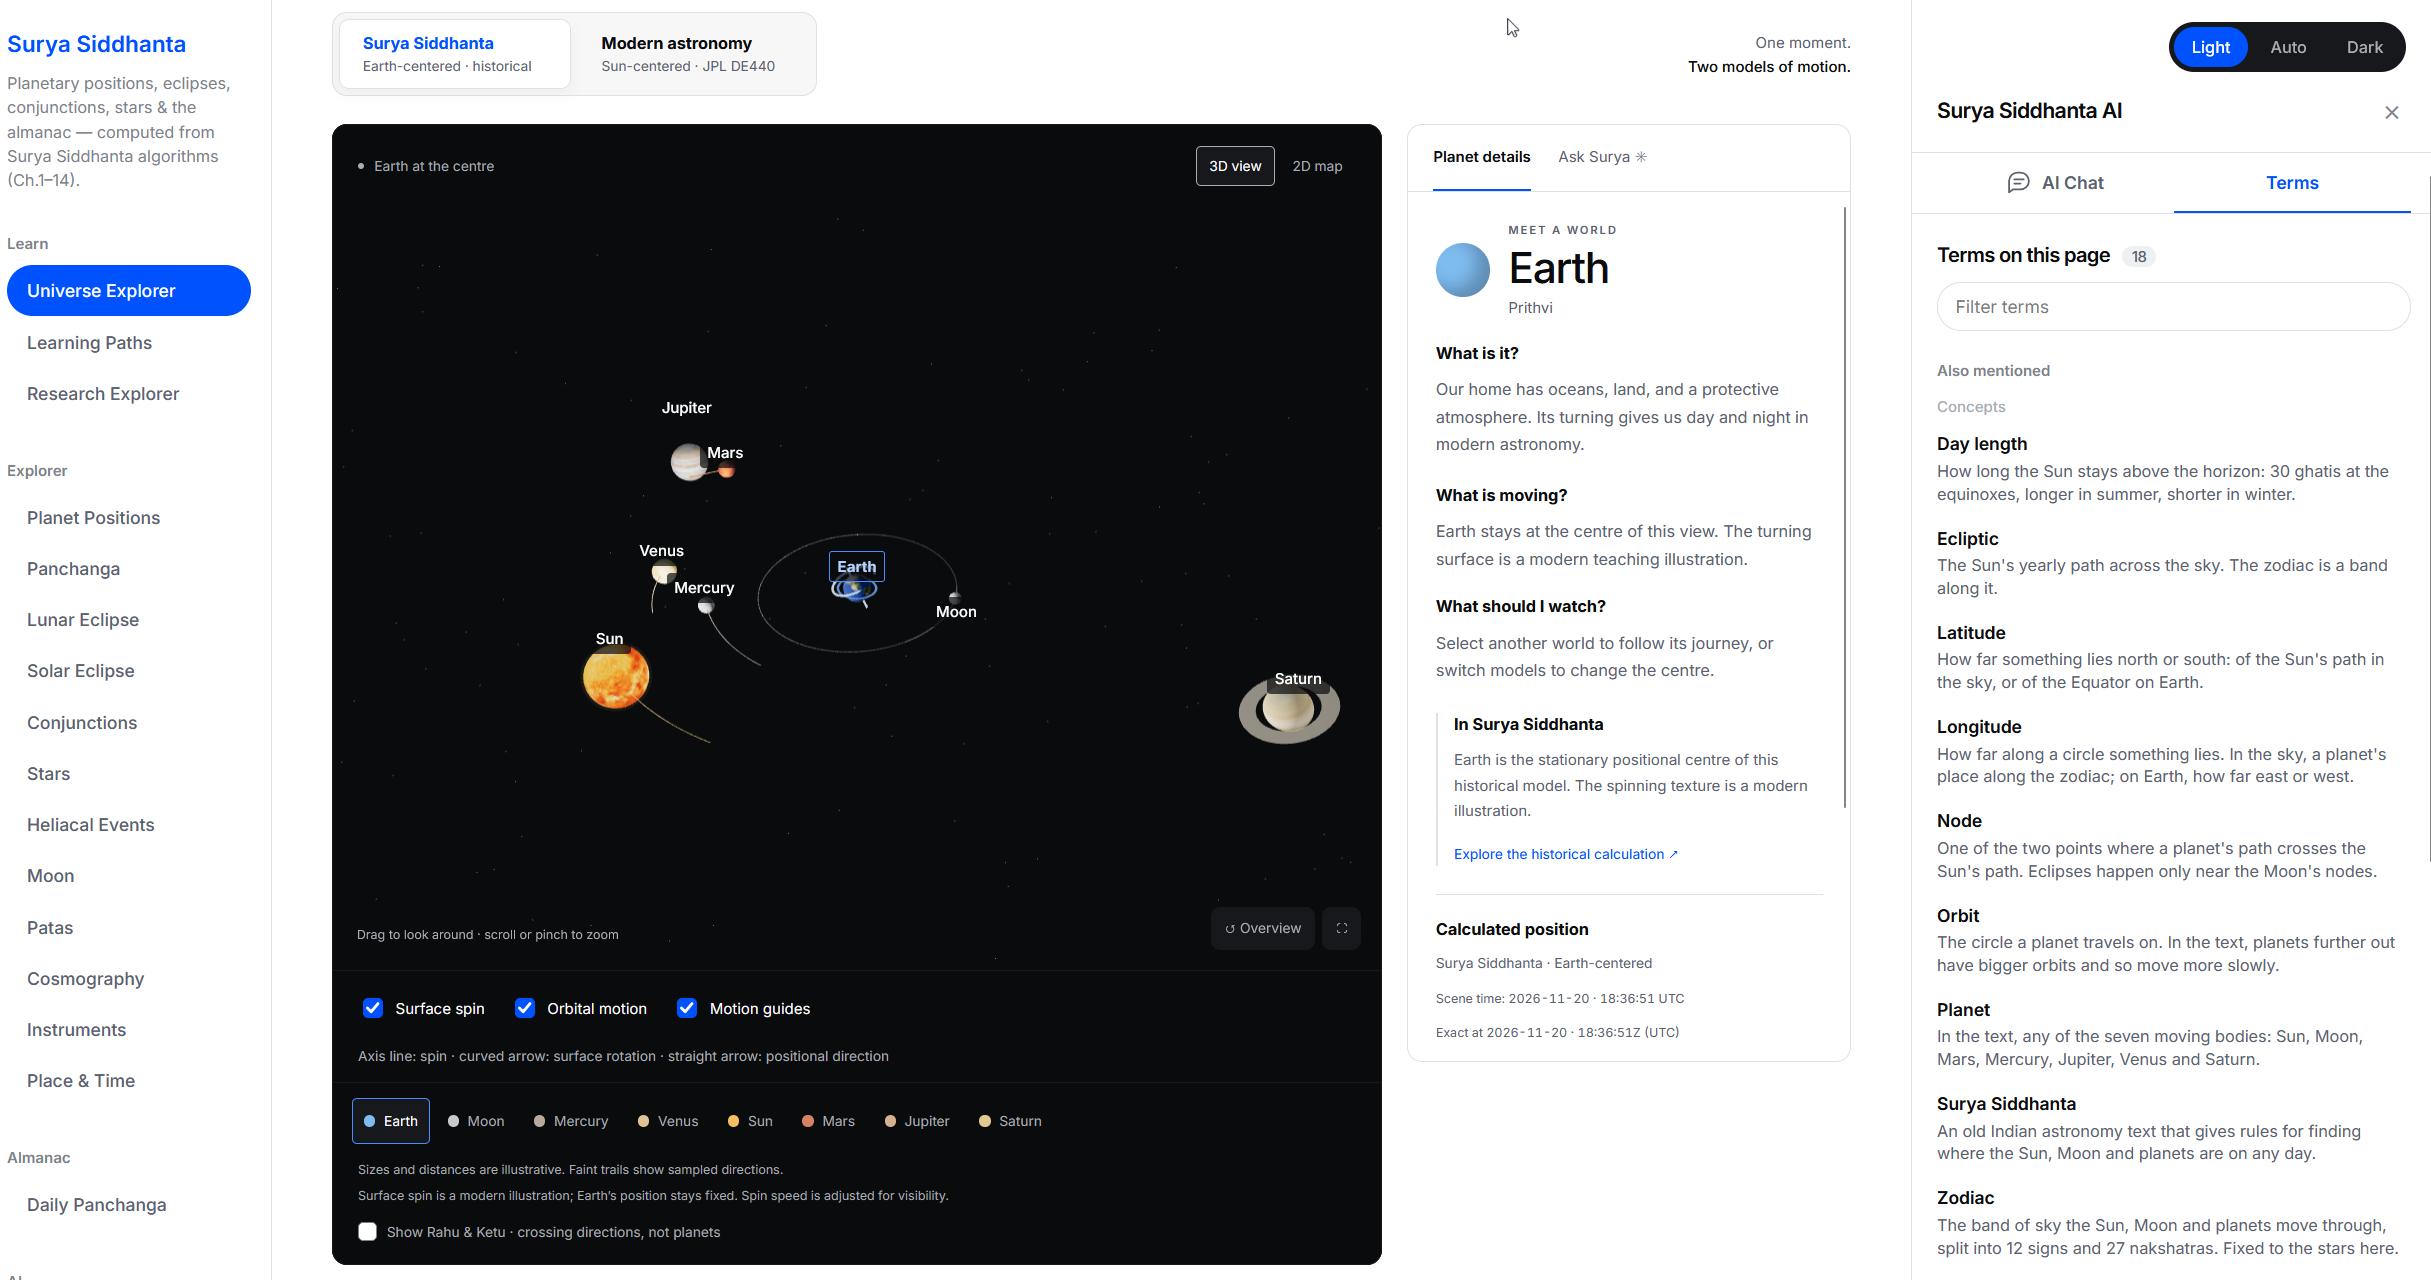
\includegraphics[width=0.95\linewidth,height=0.8\textheight,keepaspectratio]{universe-explorer.png}
  \caption{Universe Explorer}
  \label{fig:universe-explorer}
\end{figure}


\subsection{Learning Paths}

As I mentioned earlier, this covers all these planets defined in this learning path section. The /learn directory contains eight working lessons: Sun, Moon, Mars, Mercury, Venus, Jupiter, Saturn and Rahu. A learner can start with the Sun and study the Moon before tracing the planetary corrections. Any lesson can also be opened by a direct link, since no order is prescribed and no mastery is claimed.

\begin{longtable}[]{@{}
  >{\raggedright\arraybackslash}p{(\linewidth - 2\tabcolsep) * \real{0.5000}}
  >{\raggedright\arraybackslash}p{(\linewidth - 2\tabcolsep) * \real{0.5000}}@{}}
\caption{Learning paths and their implemented experiments}\label{tab:learning-paths}\\
\toprule\noalign{}
Learning path & Implemented experiment \\
\midrule\noalign{}
\endfirsthead
\caption[]{Learning paths and their implemented experiments (continued)}\\
\toprule\noalign{}
Learning path & Implemented experiment \\
\midrule\noalign{}
\endhead
\bottomrule\noalign{}
\endlastfoot
Sun & Mean and manda-corrected longitude; tropical Sun, declination and day/night length at Ujjain. \\
Moon & Two correction positions; Sun--Moon elongation, 12-degree tithi intervals and waxing/waning paksha. \\
Mars & The original five-position lesson and its saved research panel. \\
Mercury and Venus & Individual lessons and a same-date comparison of every correction stage and Sun separation. \\
Jupiter and Saturn & Individual lessons and a same-date comparison of the five-position sequence. \\
Rahu & Ascending and descending lunar nodes, regression, longitude geometry and an eclipse concept quiz. \\
\end{longtable}

All seven body lessons use the same basic structure, including date validation, a direction diagram, API-based calculation stages, chapter references, a prediction check, and JSON export. Extra panels are added depending on the topic. The Sun and Moon lessons show two positions, while the star-planets show five. Planet comparison lessons use one API response so both planets use the same input date.

The seasonal panel clearly changes from sidereal to tropical longitude and uses the library's hour-angle method for day length. The Moon panel shows elongation and tithi, where each tithi represents 12° of angular separation and may not match one civil day. For planet pairs, Sun separation means longitude difference and should not be treated as a visibility estimate.

Downloads also include lesson-specific data such as day-length values, tithi results, or planet comparison rows. The interface prevents old responses from replacing newer ones. If a request fails or is invalid, export is disabled and any previous result is marked clearly. The numerical lessons still work even if the optional corpus is unavailable.

\subsubsection{Mars Learning Lab}

We created a learn path for all planets, here in the image mars presents the Chapter 2 true-place calculation as an interactive learning activity for Mars. The user selects a date and can move through a 90-day range before or after it is using a slider. The existing book API performs the calculations at midnight in Ujjain mean time. The results are shown as sidereal angular positions of Mars as seen from Earth. The visualization represents angles only and does not show actual orbital distances.

\begin{figure}[htbp]
  \centering
  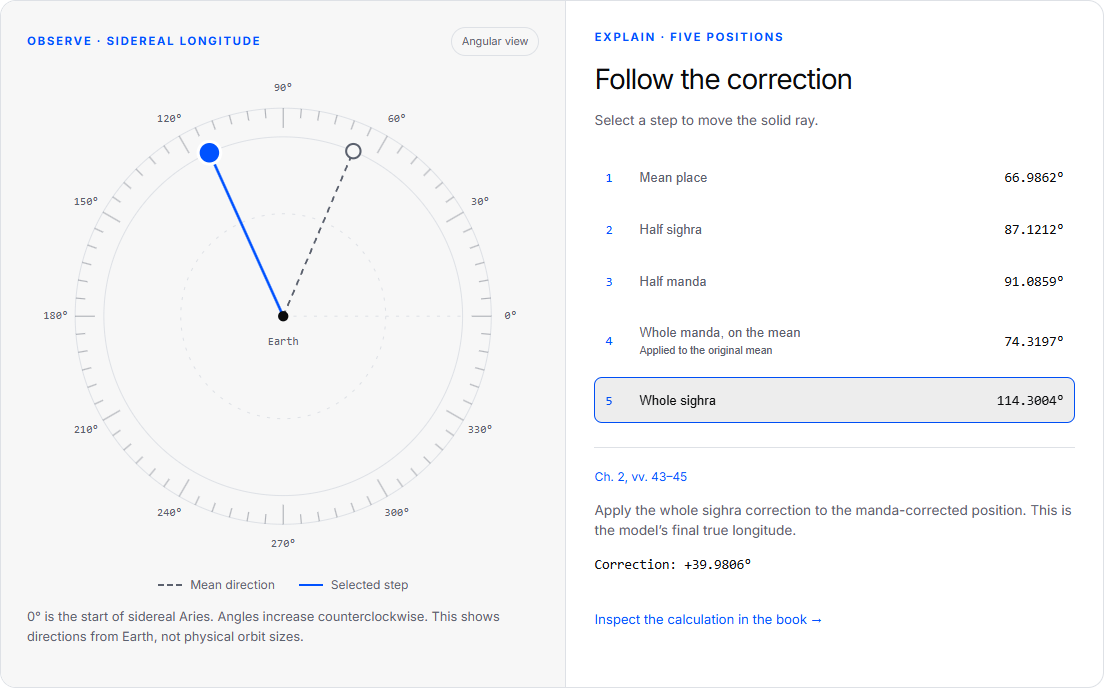
\includegraphics[width=0.95\linewidth,height=0.8\textheight,keepaspectratio]{current-report-1.png}
  \caption{Mars Learning Lab showing the final correction stage for 4 November 2026}
  \label{fig:current-report-1}
\end{figure}

The learning path showing five positions: mean place, half \emph{sighra}, half \emph{manda}, whole \emph{manda} applied to the original mean, and whole \emph{sighra}. The fourth step again uses the original mean, so these steps should not be treated as a simple cumulative addition. For the demonstration date, the final longitude is 114.3004°.

A link opens the main calculation using the same date while optional corpus text is shown separately from the calculation so users can check how the values are calculated. We are also checking whether the final position is ahead of or behind the mean using the shortest angular separation. The JSON export stores the inputs, time basis, coordinate frame, and intermediate results. We implemented this feature for learning purposes, but its impact on student learning has not yet been evaluated.


\subsection{Research Explorer}

We also developed a research explorer to visualise the results of the longitude comparison study. The /research page displays the stored comparison results for the Sun, Moon, Mercury, Venus, Mars, Jupiter, Saturn and Rahu across eleven consecutive 100-year periods from 1550 to 2649 CE. In this study, Rahu represents the ascending node of the Moon's orbit. Users can select a celestial body and time period using either an 8 × 11 root mean square (RMS) error matrix or separate selection controls. For each selection, the naive and time-aligned results are displayed using the same vertical-axis scale, allowing users to compare the differences between the two methods.

\begin{figure}[htbp]
  \centering
  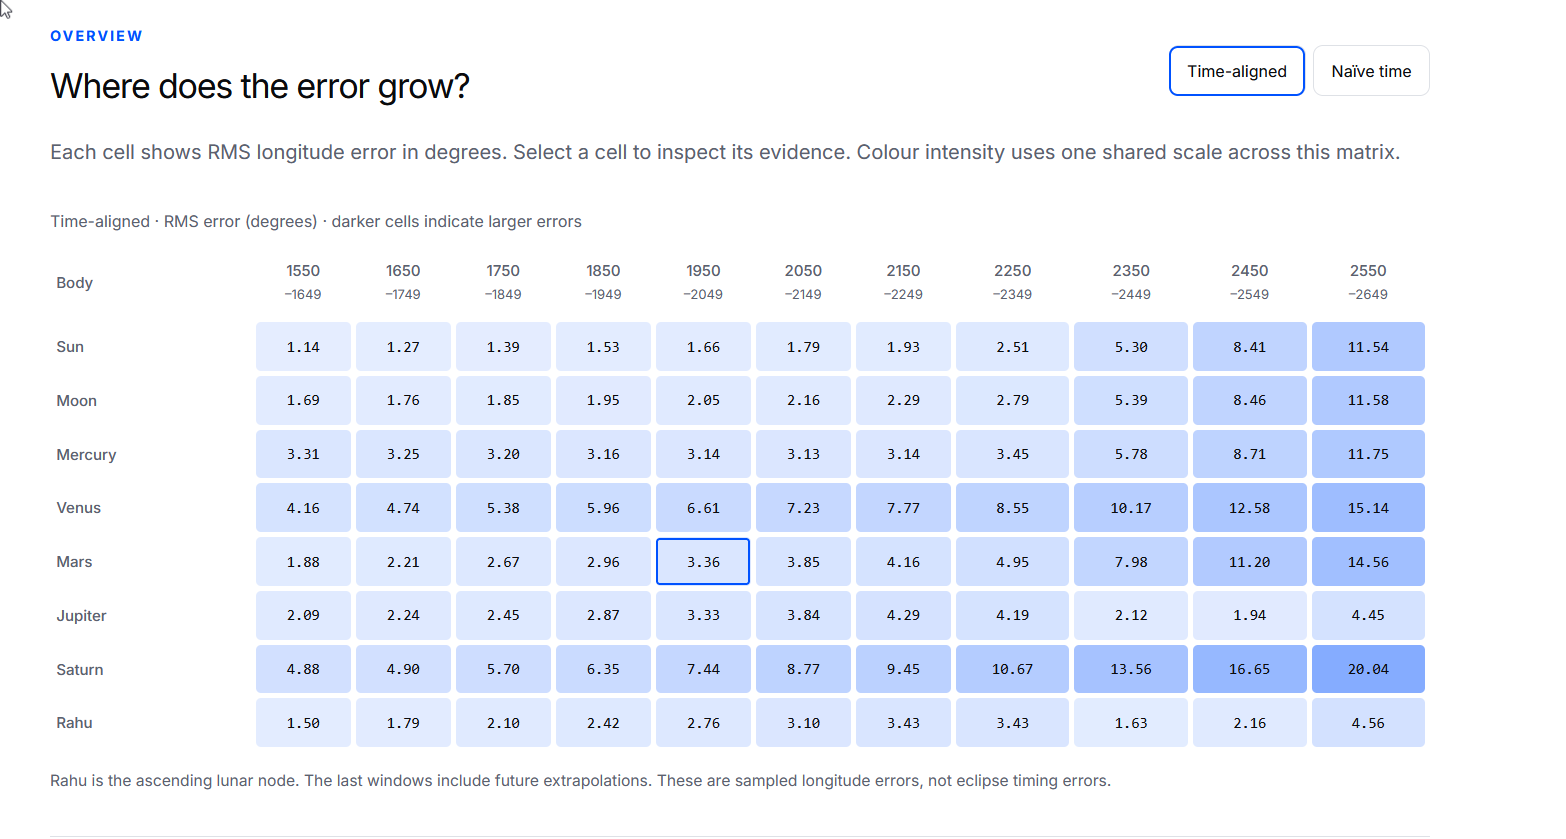
\includegraphics[width=0.95\linewidth,height=0.8\textheight,keepaspectratio]{research-matrix.png}
  \caption{Time-aligned RMS longitude errors from the saved DE440 comparison}
  \label{fig:research-matrix}
\end{figure}

In the naive method, the Julian Date (JD) obtained from the library is directly treated as Terrestrial Time (TT) for comparison with modern ephemeris data. The time-aligned method first applies a meridian correction by subtracting 75.7873°/360 days and then adds the approximate ΔT correction used in the evaluation~\cite{espenak2006,nigam2026de440}. This adjustment changes only the time used for the reference ephemeris, while the historical calculation formulas and constants remain unchanged. For the Moon, during 1550--1649, the recorded root mean square (RMS) longitude error decreased from 3.990° to 1.686°. This improvement shows the effect of time alignment on the comparison and should not be considered a calibration of the \emph{\surya} model.


\subsection{Explorer Menu}

\textbf{Planet Positions} (Chapters 1 and 2) is the home page. It takes
a date and time zone and seven checkboxes to choose among Sun,
Moon, Mars, Mercury, Jupiter, Venus and Saturn. A line above the
results gives the Julian Day in Ujjain mean time, the ahargana and the
ayanamsha. The table lists each body, the true and mean sidereal
longitude, the tropical longitude, the rashi with degrees and the
nakshatra with its pada. Below it, an interactive SVG zodiac wheel
plots the selected bodies on the twelve signs.

\begin{figure}[htbp]
  \centering
  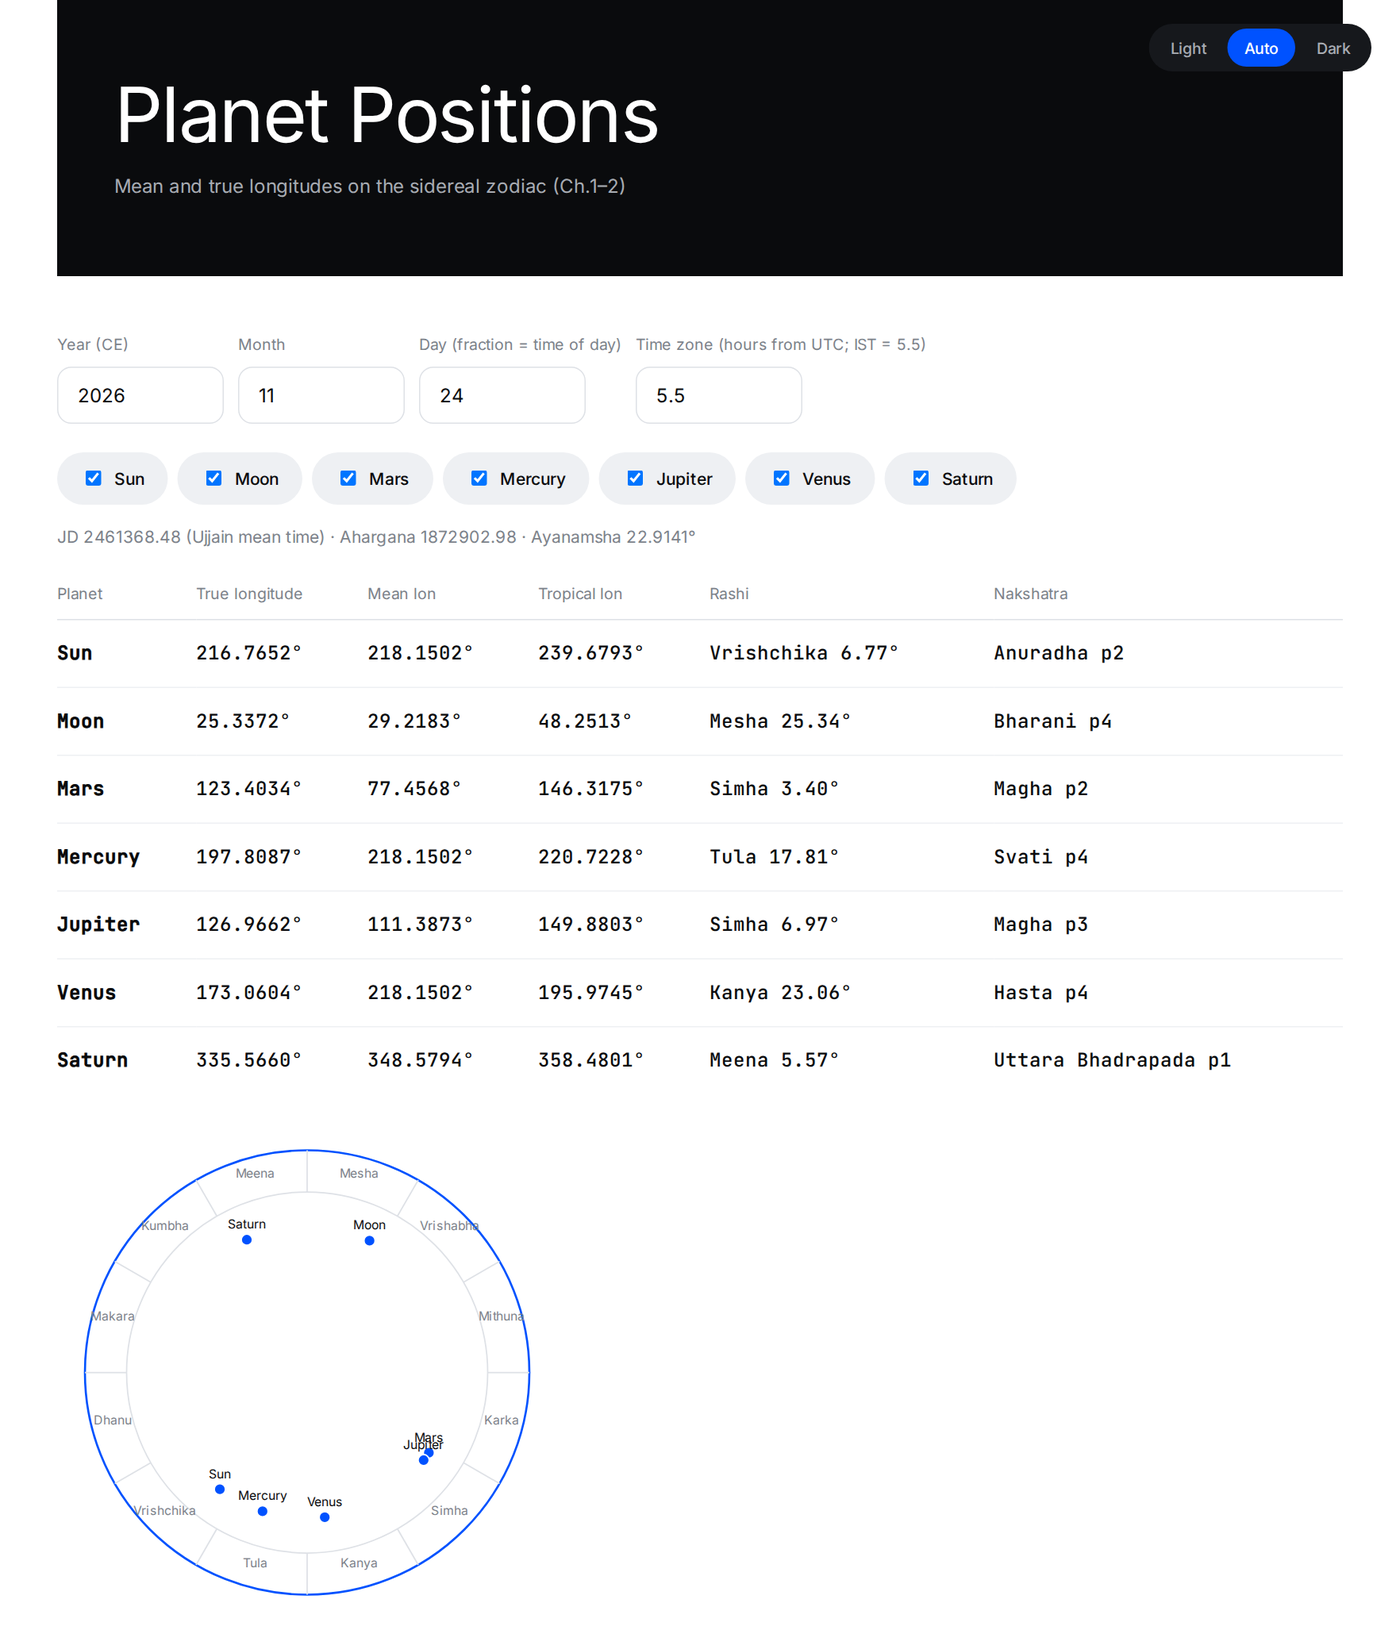
\includegraphics[width=\linewidth,height=0.62\textheight,keepaspectratio]{ui/ui-positions.png}
  \caption{Planet Positions: longitudes table and zodiac wheel}
  \label{fig:ui-positions}
\end{figure}

\textbf{Panchanga} gives the calendar elements for one moment: tithi,
vara, nakshatra, yoga, karana, lunar month (masa), season (ritu) and
the year of the sixty-year cycle (samvatsara), together with the Sun's
and Moon's longitudes and the ayanamsha. Because tithi and nakshatra
change during the day, this page takes a clock time as well as a date.

\begin{figure}[htbp]
  \centering
  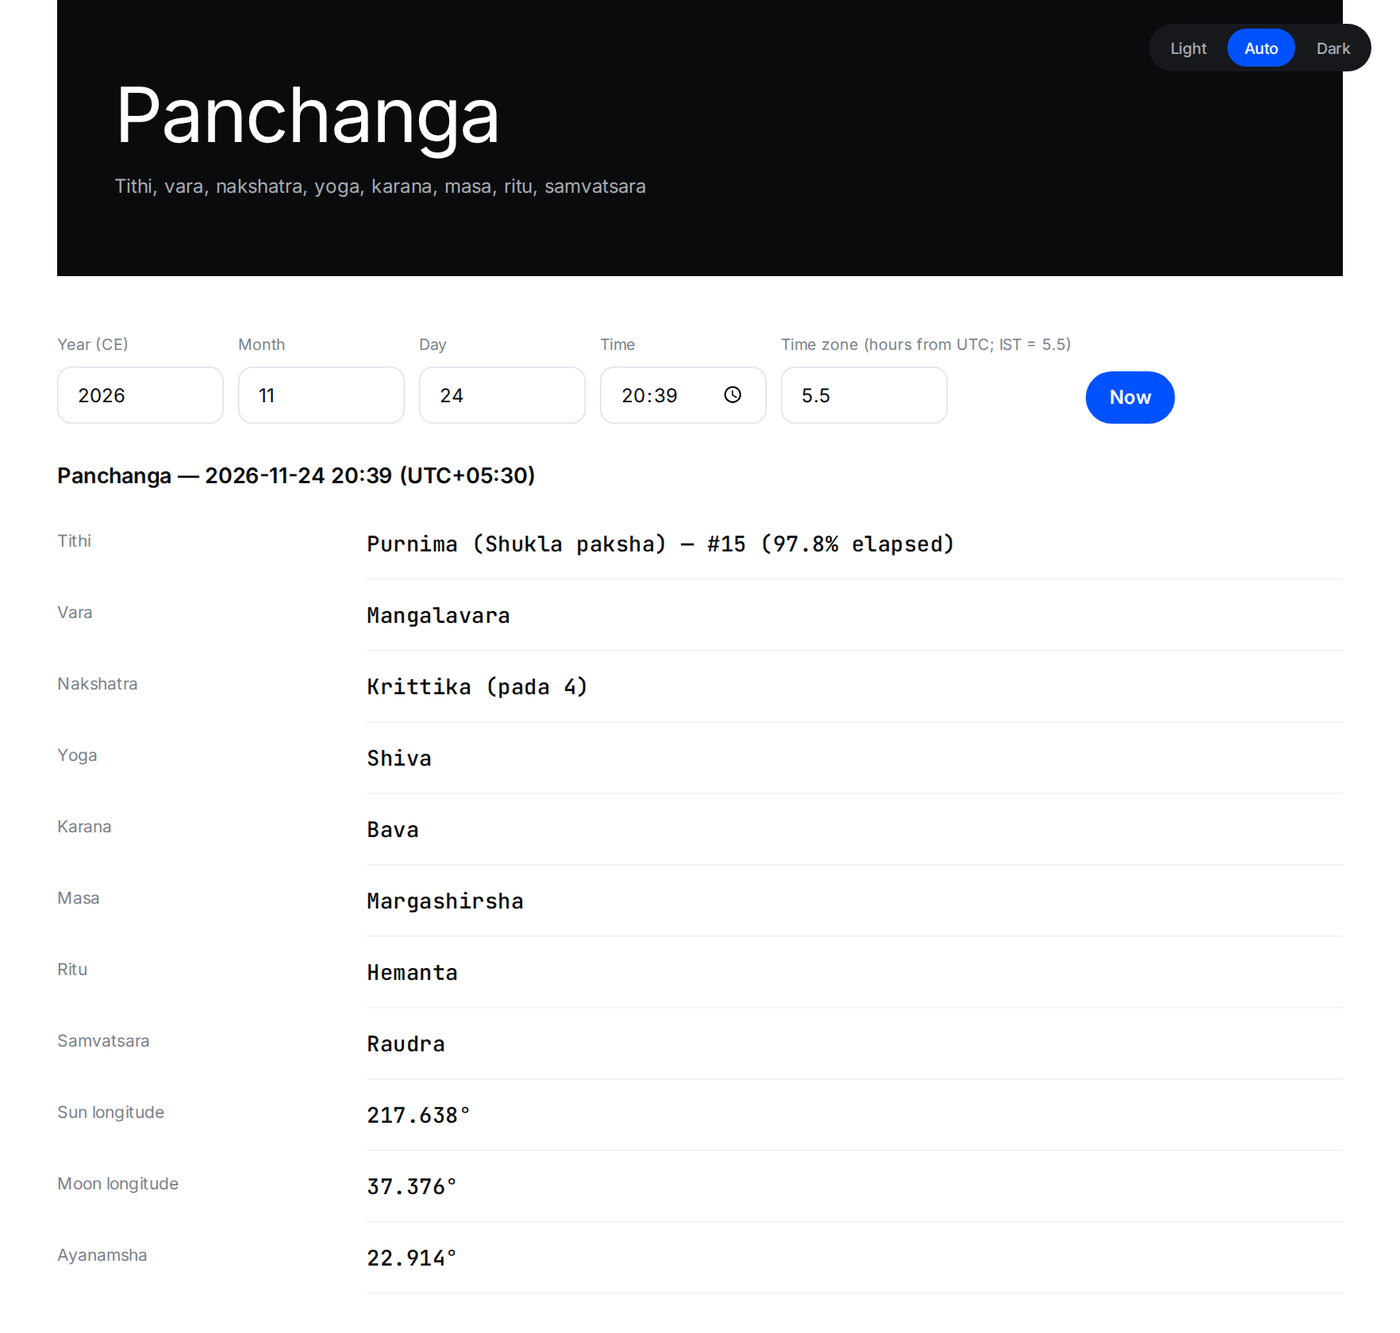
\includegraphics[width=\linewidth,height=0.62\textheight,keepaspectratio]{ui/ui-panchanga.png}
  \caption{Panchanga for a chosen date and clock time}
  \label{fig:ui-panchanga}
\end{figure}

\textbf{Lunar Eclipse} (Chapter 4) takes a date and reports whether an
eclipse occurs at the nearest full moon. When there is one, the table
gives its type and magnitude, the Moon's latitude, the diameters of the
Moon and the earth's shadow in arc-minutes, the half-duration and for
a total eclipse, the half-duration of totality, with a summary
sentence. The page reminds the user to choose a date near full moon.

\begin{figure}[htbp]
  \centering
  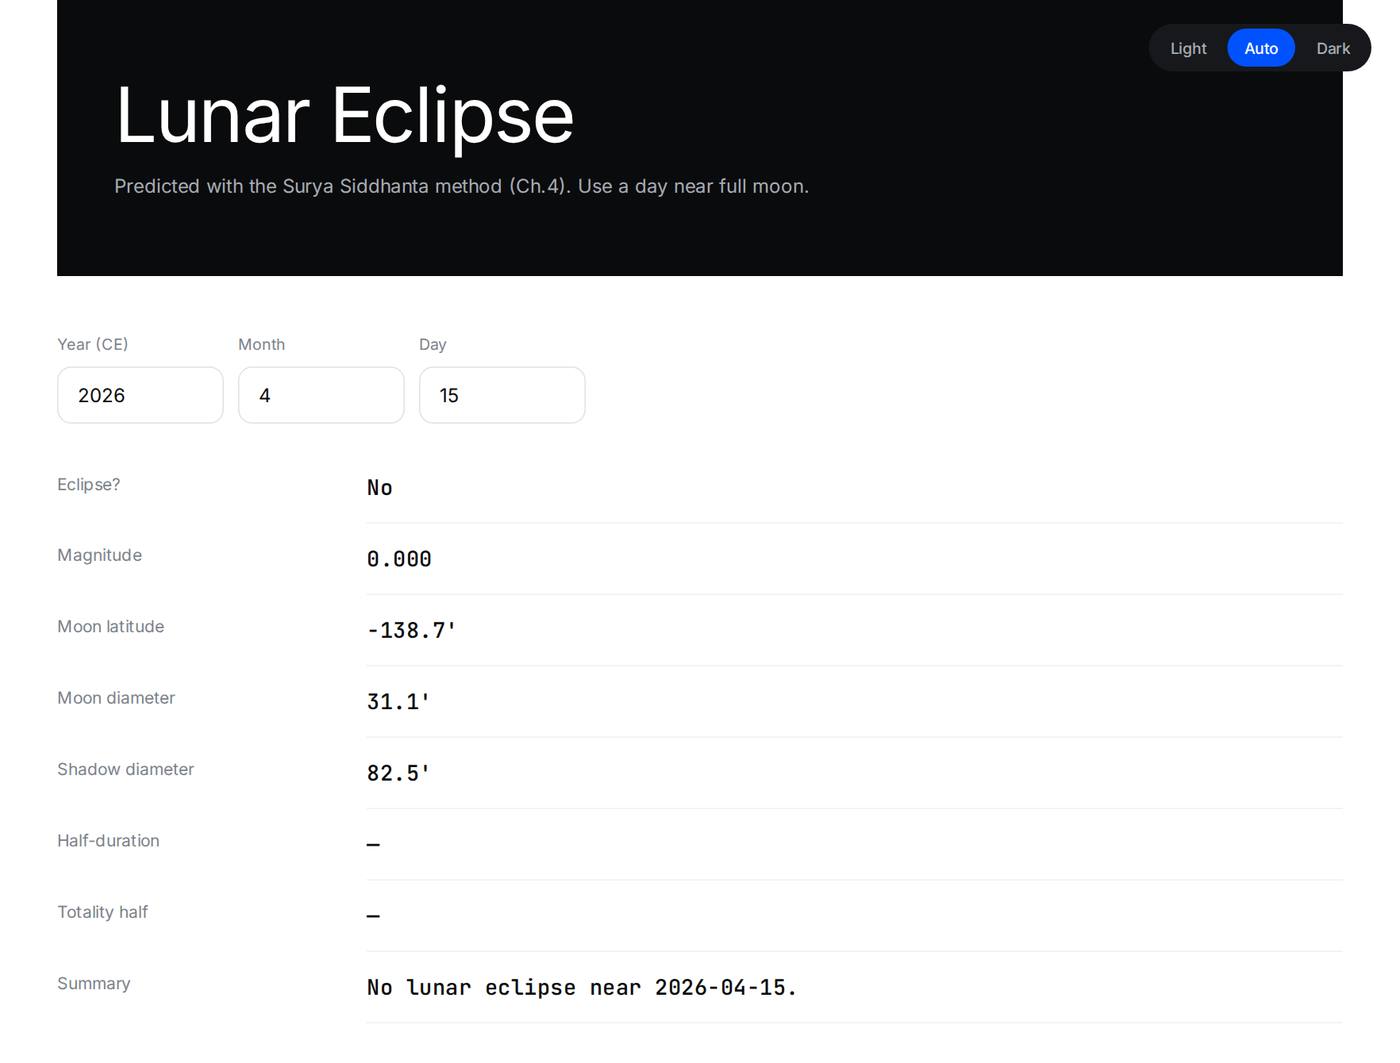
\includegraphics[width=\linewidth,height=0.62\textheight,keepaspectratio]{ui/ui-lunar-eclipse.png}
  \caption{Lunar Eclipse page}
  \label{fig:ui-lunar-eclipse}
\end{figure}

\textbf{Solar Eclipse} (Chapter 5) adds the observer's latitude and
longitude, because a solar eclipse depends on where it is seen from.
Besides type, magnitude and the two disc diameters, it reports the
parallax in longitude (lambana) and in latitude (nati), the
half-duration, the Sun's altitude at conjunction and whether the
eclipse is visible from the chosen place. An eclipse with the Sun below
the horizon is reported as not visible.

\begin{figure}[htbp]
  \centering
  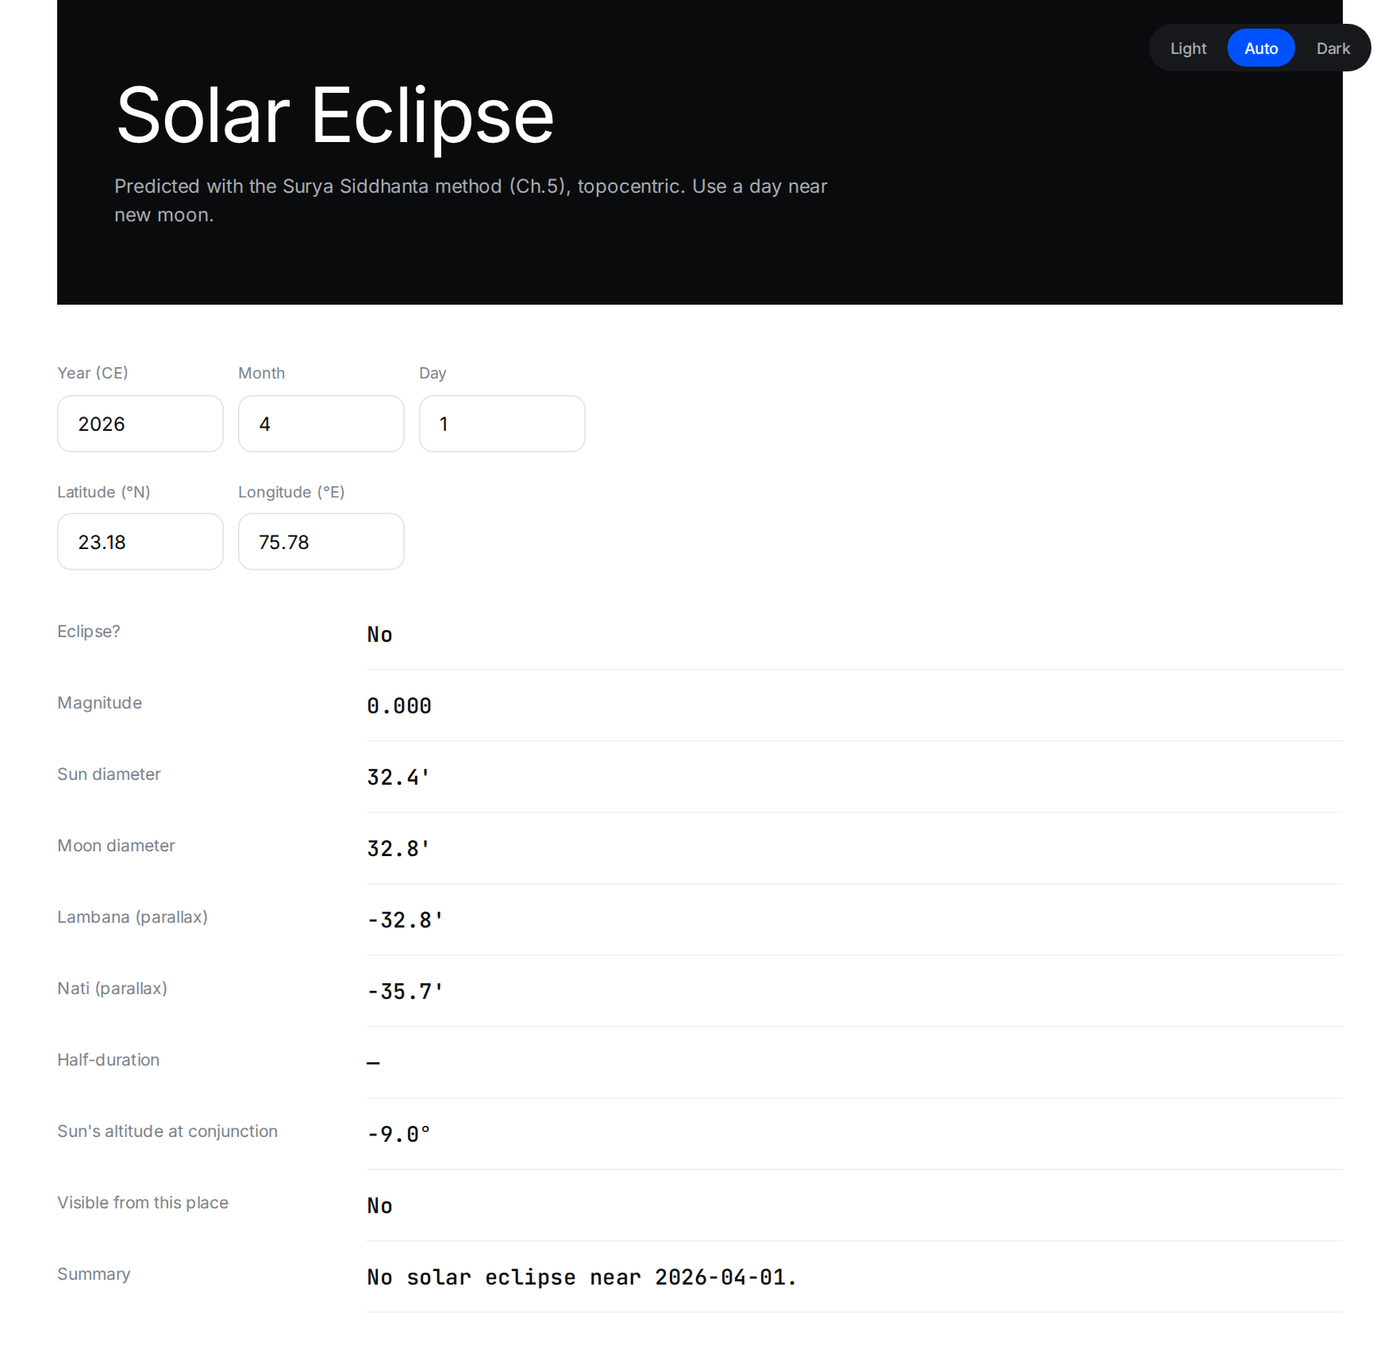
\includegraphics[width=\linewidth,height=0.62\textheight,keepaspectratio]{ui/ui-solar-eclipse.png}
  \caption{Solar Eclipse page with the observer's place}
  \label{fig:ui-solar-eclipse}
\end{figure}

\textbf{Conjunctions} (Chapter 7) searches for meetings of two bodies.
The user picks the two from drop-down lists, enters a start year and a
span of 1 to 60 months and presses Search. The result is a summary and
a table giving the date, longitude, separation in degrees and type of
each conjunction found.

\begin{figure}[htbp]
  \centering
  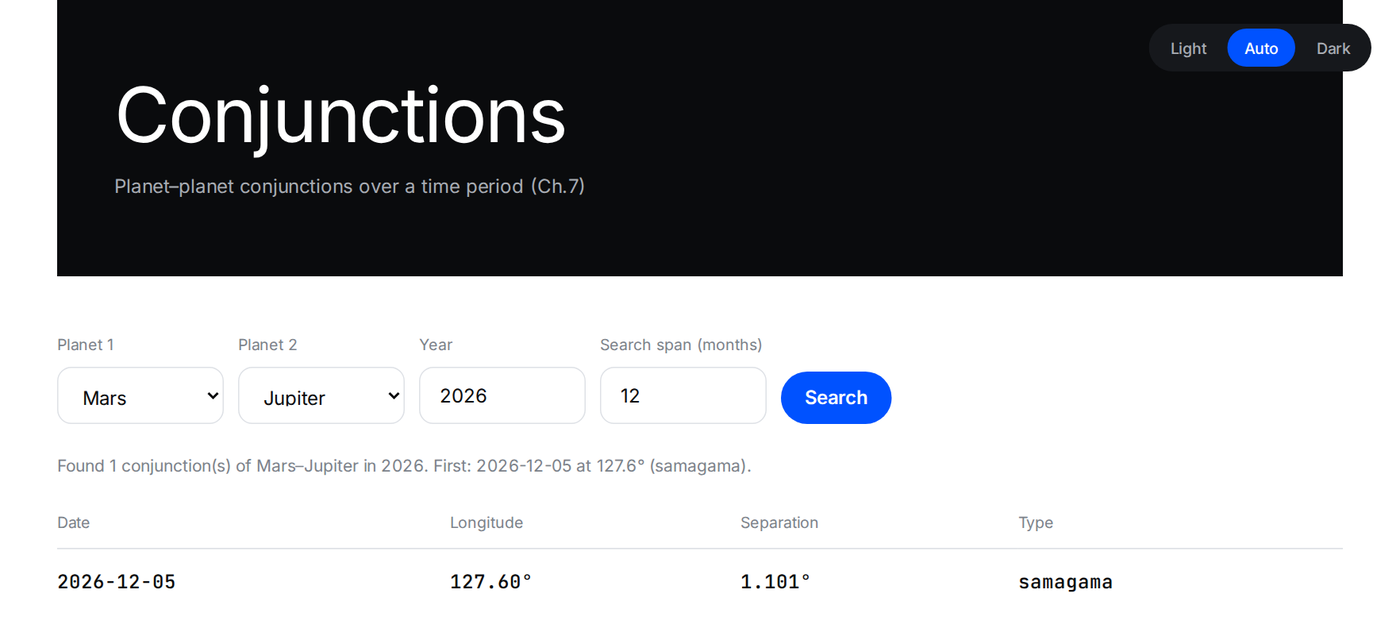
\includegraphics[width=\linewidth,height=0.62\textheight,keepaspectratio]{ui/ui-conjunctions.png}
  \caption{Conjunctions search for Mars and Jupiter over twelve months}
  \label{fig:ui-conjunctions}
\end{figure}

\textbf{Stars} (Chapter 8) covers the twenty-seven nakshatras. A
drop-down list chooses one, and the page shows its name in Devanagari,
its junction star (yogatara), deity and gana, its span on the ecliptic,
the star's sidereal longitude and latitude, tropical longitude, right
ascension and declination and its rising and setting. A sky map in SVG
plots all the junction stars and highlights the chosen one.

\begin{figure}[htbp]
  \centering
  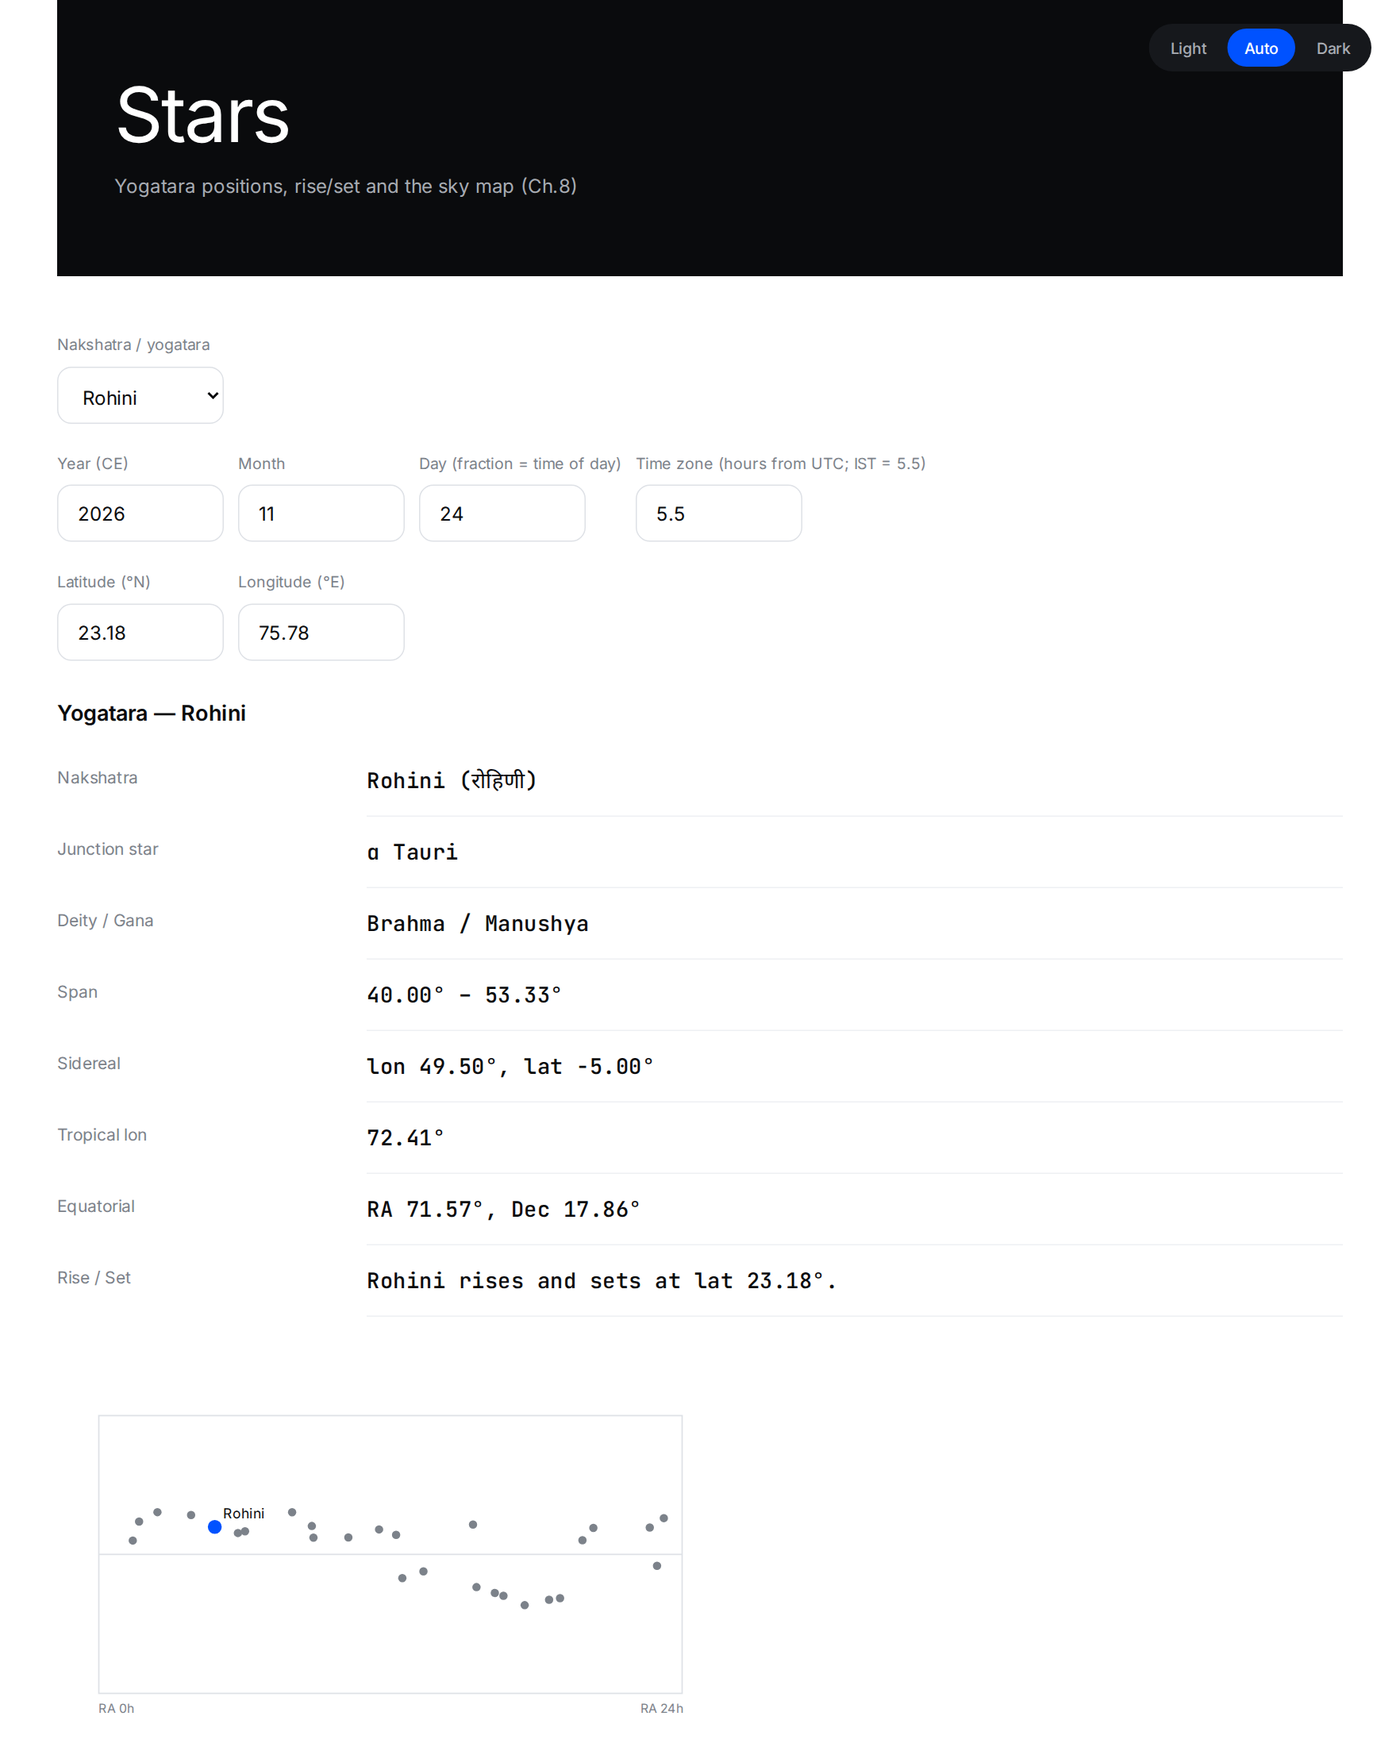
\includegraphics[width=\linewidth,height=0.62\textheight,keepaspectratio]{ui/ui-stars.png}
  \caption{Stars page with the nakshatra details and sky map}
  \label{fig:ui-stars}
\end{figure}

\textbf{Heliacal Events} (Chapter 9) lists when Mars, Mercury, Jupiter,
Venus or Saturn first becomes visible after conjunction with the Sun,
or last visible before it. The inputs are the planet, a start year and
a span of up to 36 months. Each row gives the date, the event, the
elongation from the Sun and whether the event is in the east or the
west.

\begin{figure}[htbp]
  \centering
  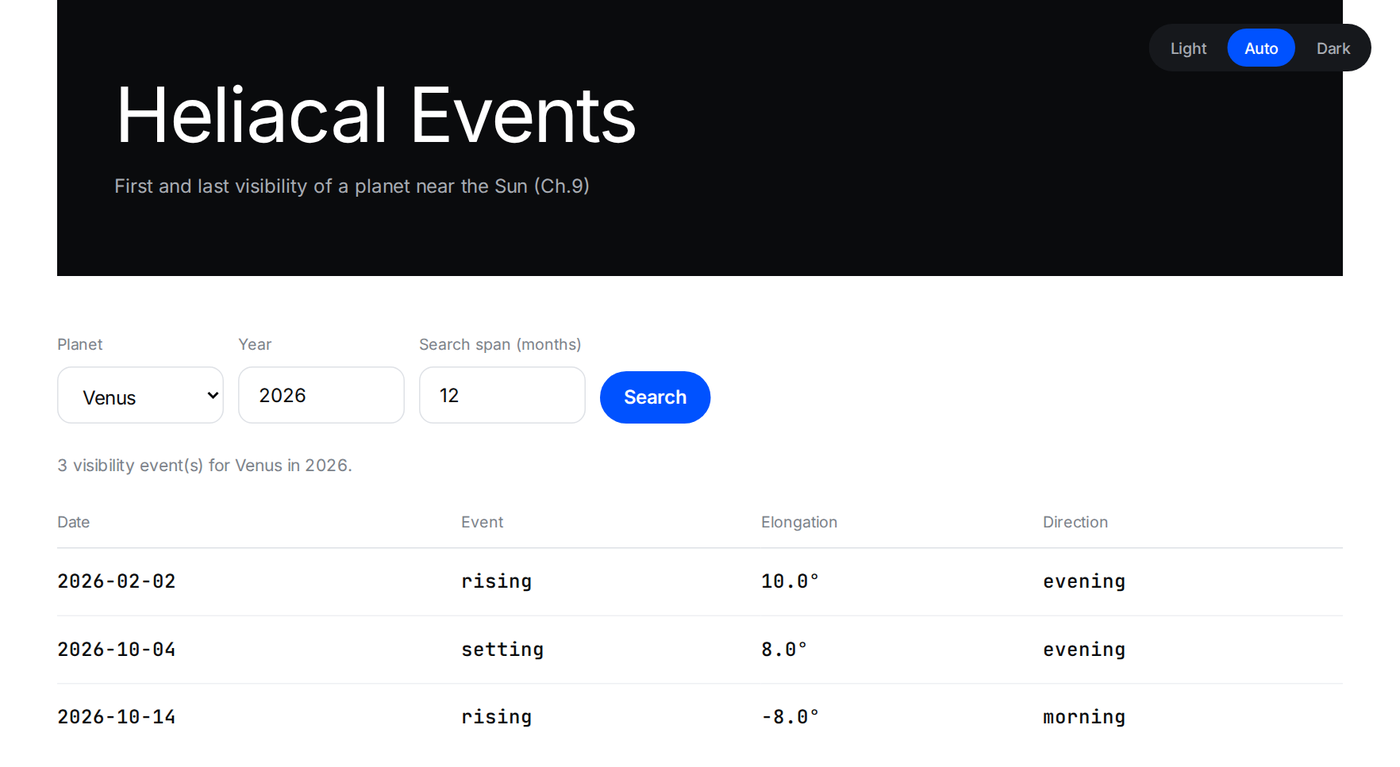
\includegraphics[width=\linewidth,height=0.62\textheight,keepaspectratio]{ui/ui-heliacal.png}
  \caption{Heliacal Events search results}
  \label{fig:ui-heliacal}
\end{figure}

\textbf{Moon} (Chapter 10) takes a date, time zone and place. It gives
the phase name and whether the Moon is waxing or waning, the
illuminated percentage, the elongation from the Sun, the width of the
crescent (bahu), the angle of the bright limb, the tilt of the horns
(valana), and the times of moonrise and moonset in the chosen zone.

\begin{figure}[htbp]
  \centering
  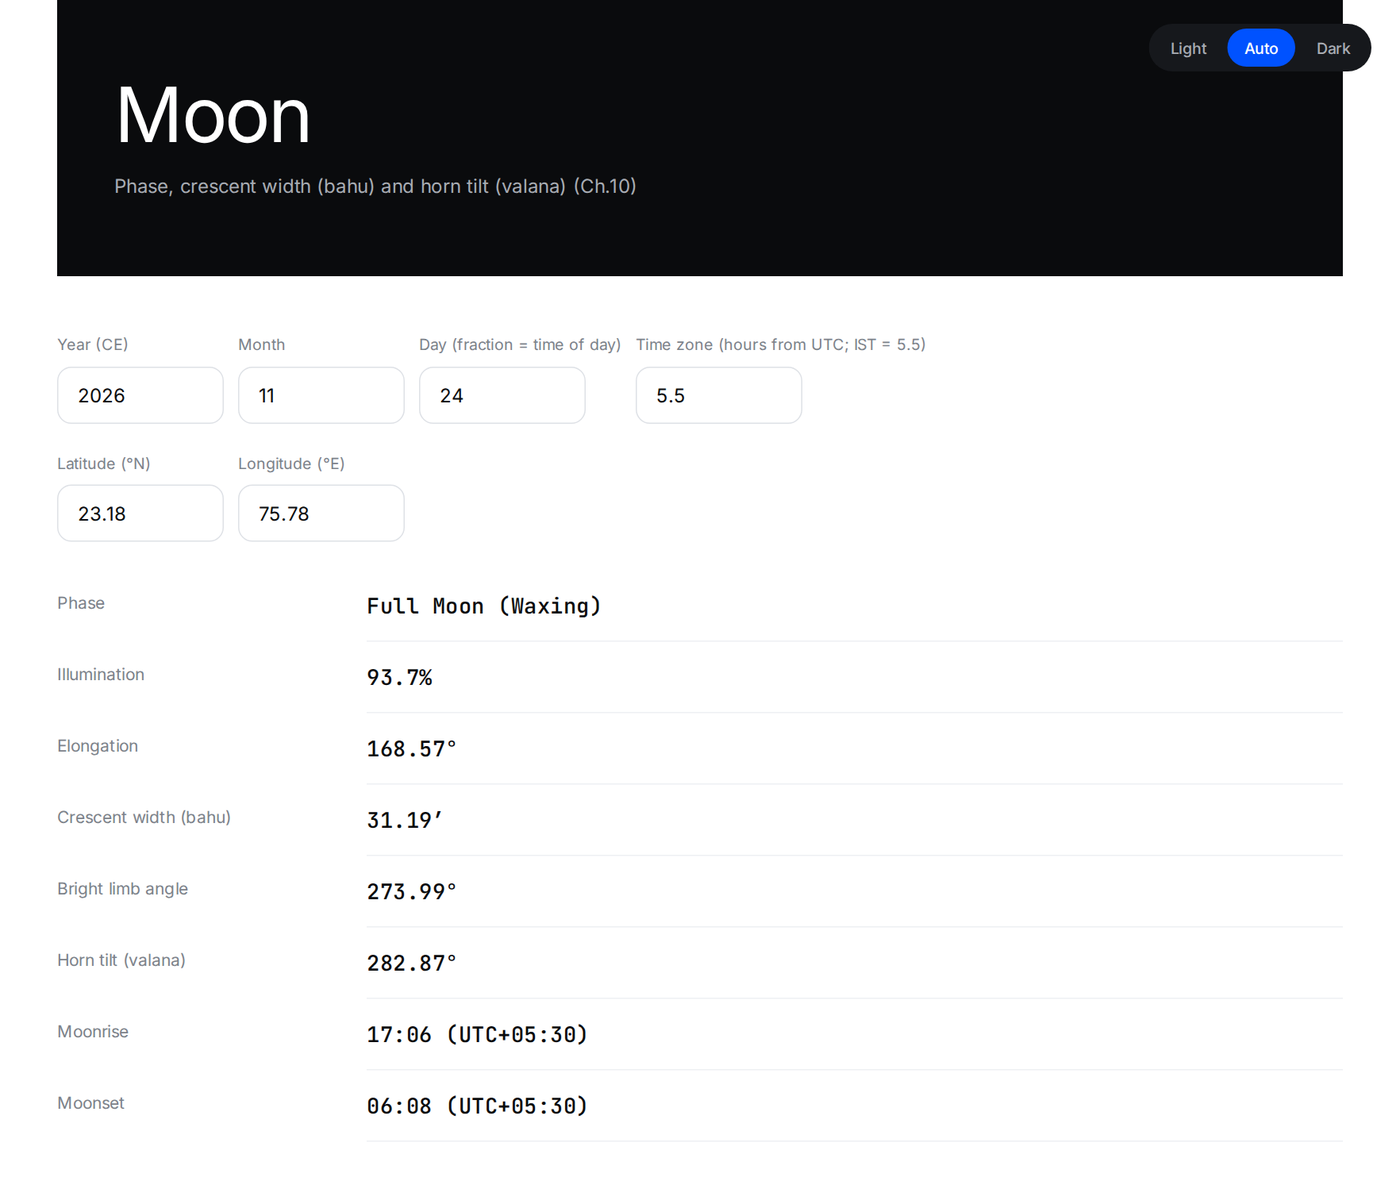
\includegraphics[width=\linewidth,height=0.62\textheight,keepaspectratio]{ui/ui-moon.png}
  \caption{Moon page: phase, crescent, horns, moonrise and moonset}
  \label{fig:ui-moon}
\end{figure}

\textbf{Patas} (Chapter 11) finds Vyatipata and Vaidhrita, the moments
when the Sun's and Moon's declinations are equal in amount. The user
enters a start date and a window of 7 to 365 days. Each event found
shows when it begins, its middle and its end, its duration in ghatis
and the nominal time from the sum-of-longitudes rule.

\begin{figure}[htbp]
  \centering
  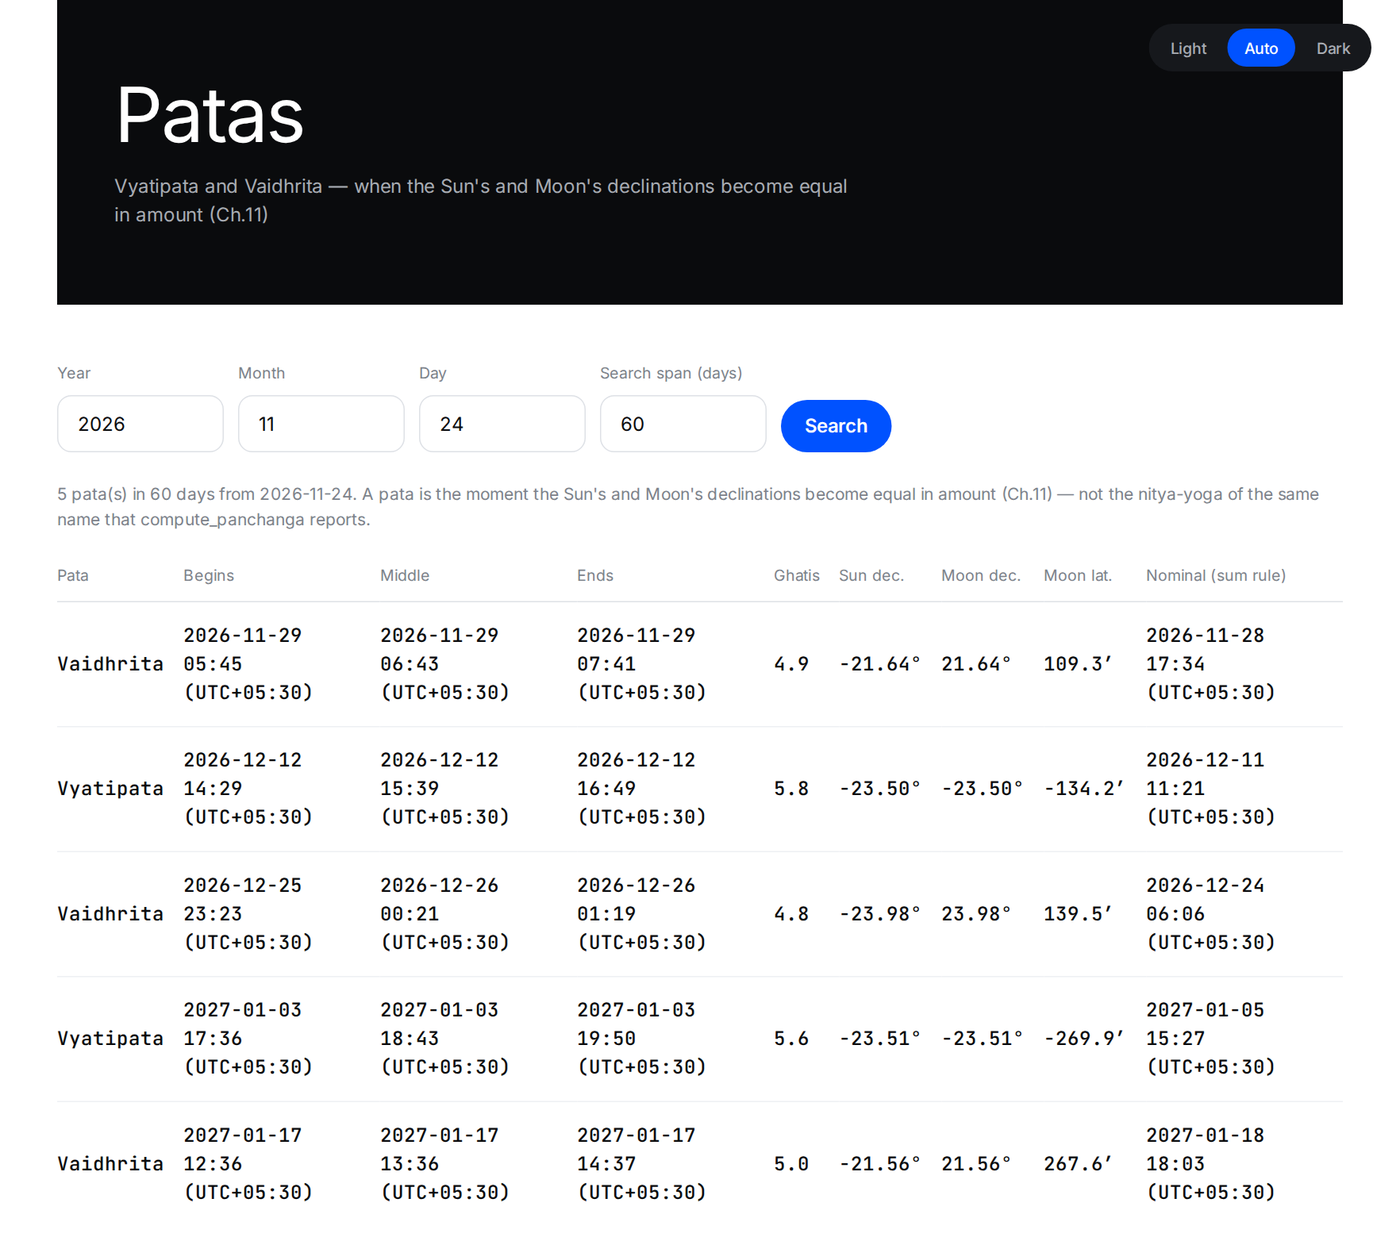
\includegraphics[width=\linewidth,height=0.62\textheight,keepaspectratio]{ui/ui-patas.png}
  \caption{Patas page listing Vyatipata and Vaidhrita events}
  \label{fig:ui-patas}
\end{figure}

\textbf{Cosmography} (Chapter 12) has four tabs because most of this
chapter is fixed dimensions rather than calculations over time.
``Earth \& Place'' takes a place and gives the earth's diameter and
circumference, the circumference corrected for latitude, the desantara
correction and the reference places on the earth. ``Orbits \&
Distances'' tabulates each planet's orbit in yojanas and the order of
the spheres. ``Cosmic Time'' takes a date and shows the elapsed part of
the current day of Brahma, the regents of the moment and the lords of
the twenty-four horas. ``Worlds'' gives the descriptive tables of the
chapter: Maya's questions, the creation, the elements, the seven
patalas and the days and nights of the orders of beings.

\begin{figure}[htbp]
  \centering
  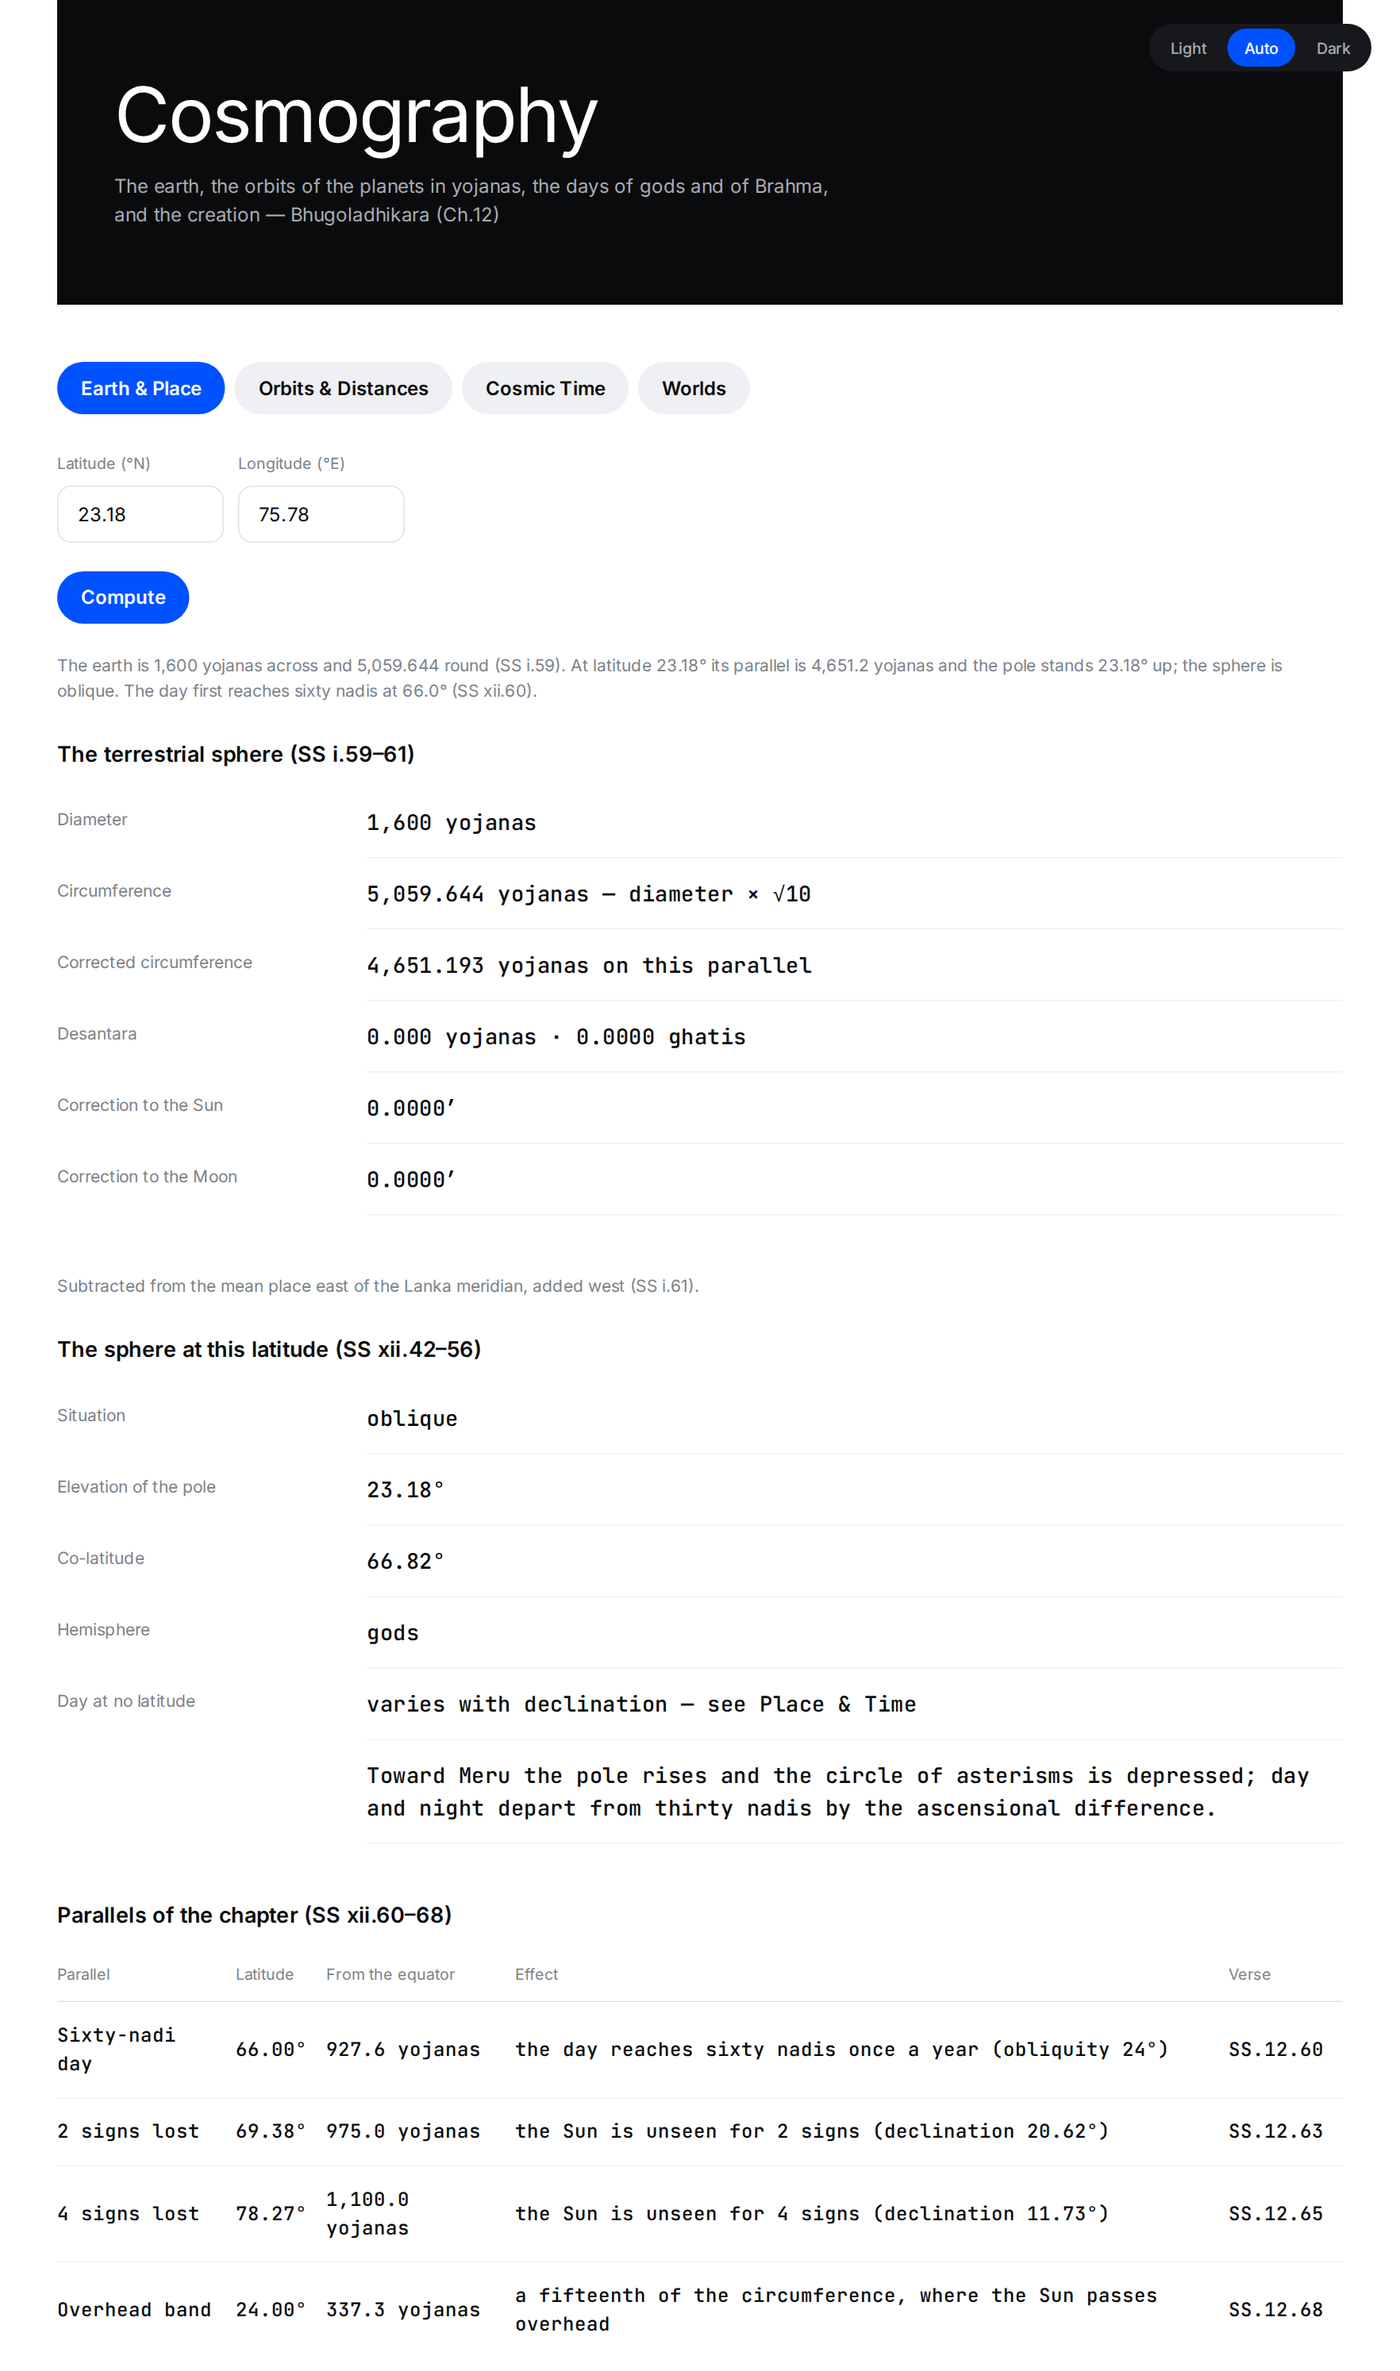
\includegraphics[width=\linewidth,height=0.62\textheight,keepaspectratio]{ui/ui-cosmography.png}
  \caption{Cosmography page, Earth \& Place tab}
  \label{fig:ui-cosmography}
\end{figure}

\textbf{Instruments} (Chapter 13) also has four tabs. ``Armillary
Sphere'' builds the sphere for a chosen date, hour and place, with
fixed stars as an option, and draws it in 3D with three.js. Checkboxes
show or hide each group of hoops and a Play button turns the sphere,
with a speed control and a slider reading the turn in ghatis. Tables
beside the sphere list the hoops, the points on the sphere and the
sines. ``Clepsydra'' models the sinking water-clock: the user sets the
number of sinkings and the current fill, converts ghatis to sinkings,
and enters an observed count of sinkings per day to see the error per
sinking. ``Shadow \& Staff'' takes the length of a gnomon's shadow and
finds the time of day with each of the four instruments the chapter
describes, so that the four answers can be compared; a shadow shorter
than the noon shadow is reported as impossible rather than as an error.
``Catalog'' lists the instruments and their parts. The 3D code loads
only when this page is opened.

\begin{figure}[htbp]
  \centering
  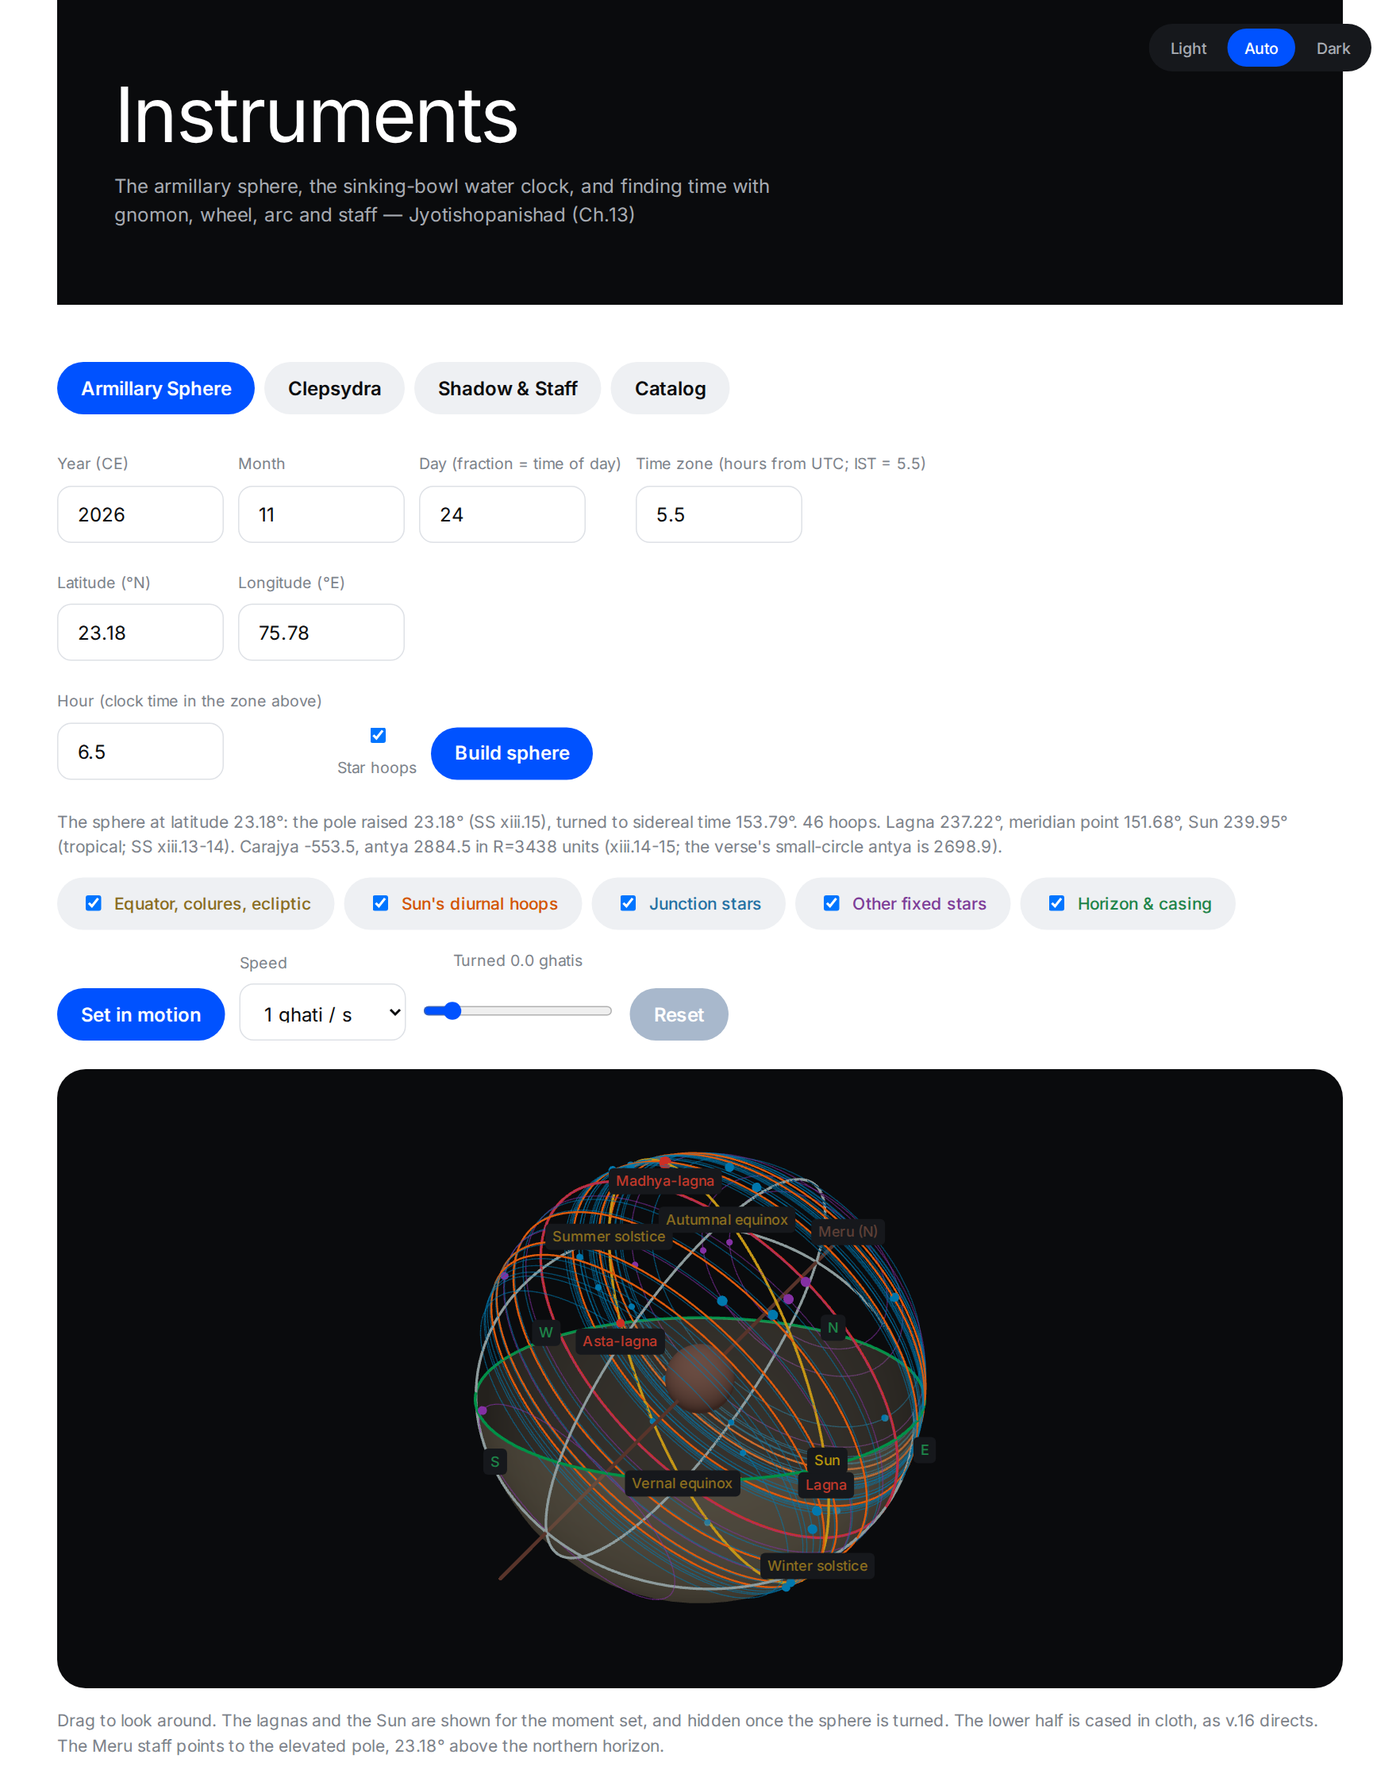
\includegraphics[width=\linewidth,height=0.62\textheight,keepaspectratio]{ui/ui-instruments.png}
  \caption{Instruments page, Armillary Sphere tab with the 3D sphere}
  \label{fig:ui-instruments}
\end{figure}

\textbf{Place \& Time} (Chapters 1 and 3) has two blocks. ``Time
Reckoning'' gives the Kali year, the years elapsed since the epoch, the
ahargana and the Julian Day. ``Direction, Place \& Time'' gives the
length of day and night, the ascendant (lagna), the gnomon shadow, the
Sun's declination and whether the Sun is below the horizon at the
chosen moment.

\begin{figure}[htbp]
  \centering
  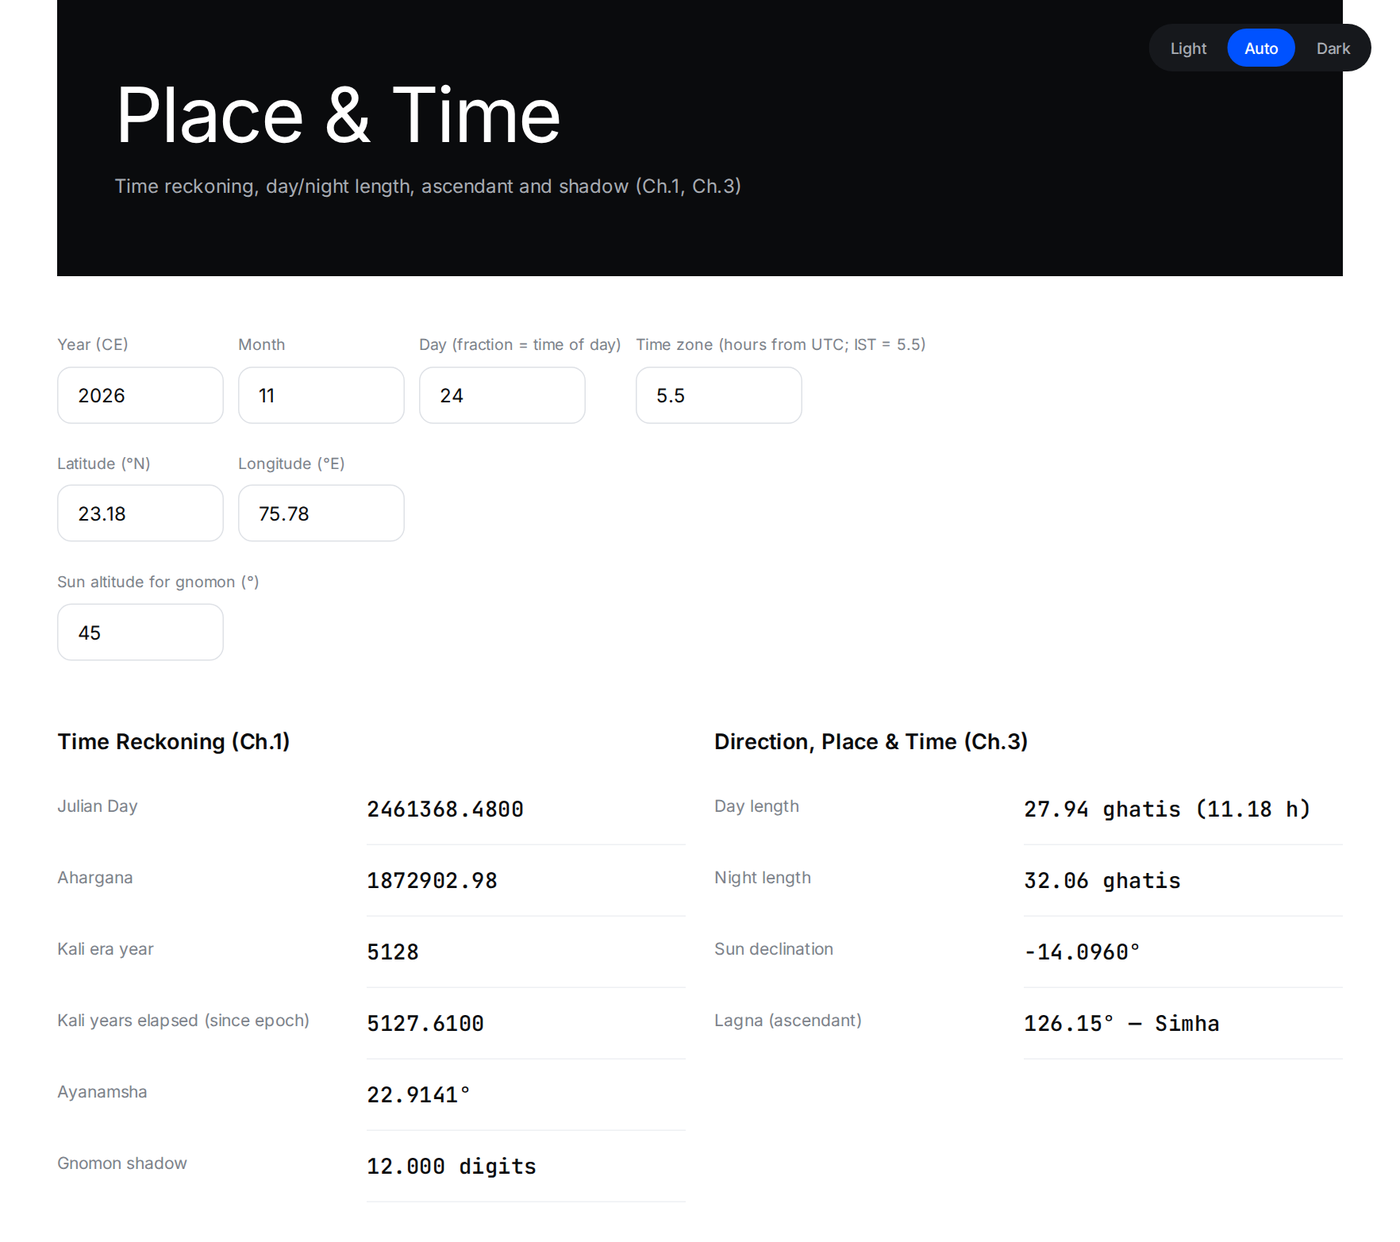
\includegraphics[width=\linewidth,height=0.62\textheight,keepaspectratio]{ui/ui-place-time.png}
  \caption{Place \& Time page}
  \label{fig:ui-place-time}
\end{figure}

\subsection{Almanac menu}

\textbf{Daily Panchanga} is the simpler almanac carried over from the
Gradio application. A card gives the five limbs (tithi, vara,
nakshatra, yoga and karana) for the chosen date, with the Sun and Moon
signs, masa, ritu, samvatsara and Moon phase. A ``Range (days)'' field
from 1 to 30 adds a table with one row per day, which can be read as a
short printed almanac.

\begin{figure}[htbp]
  \centering
  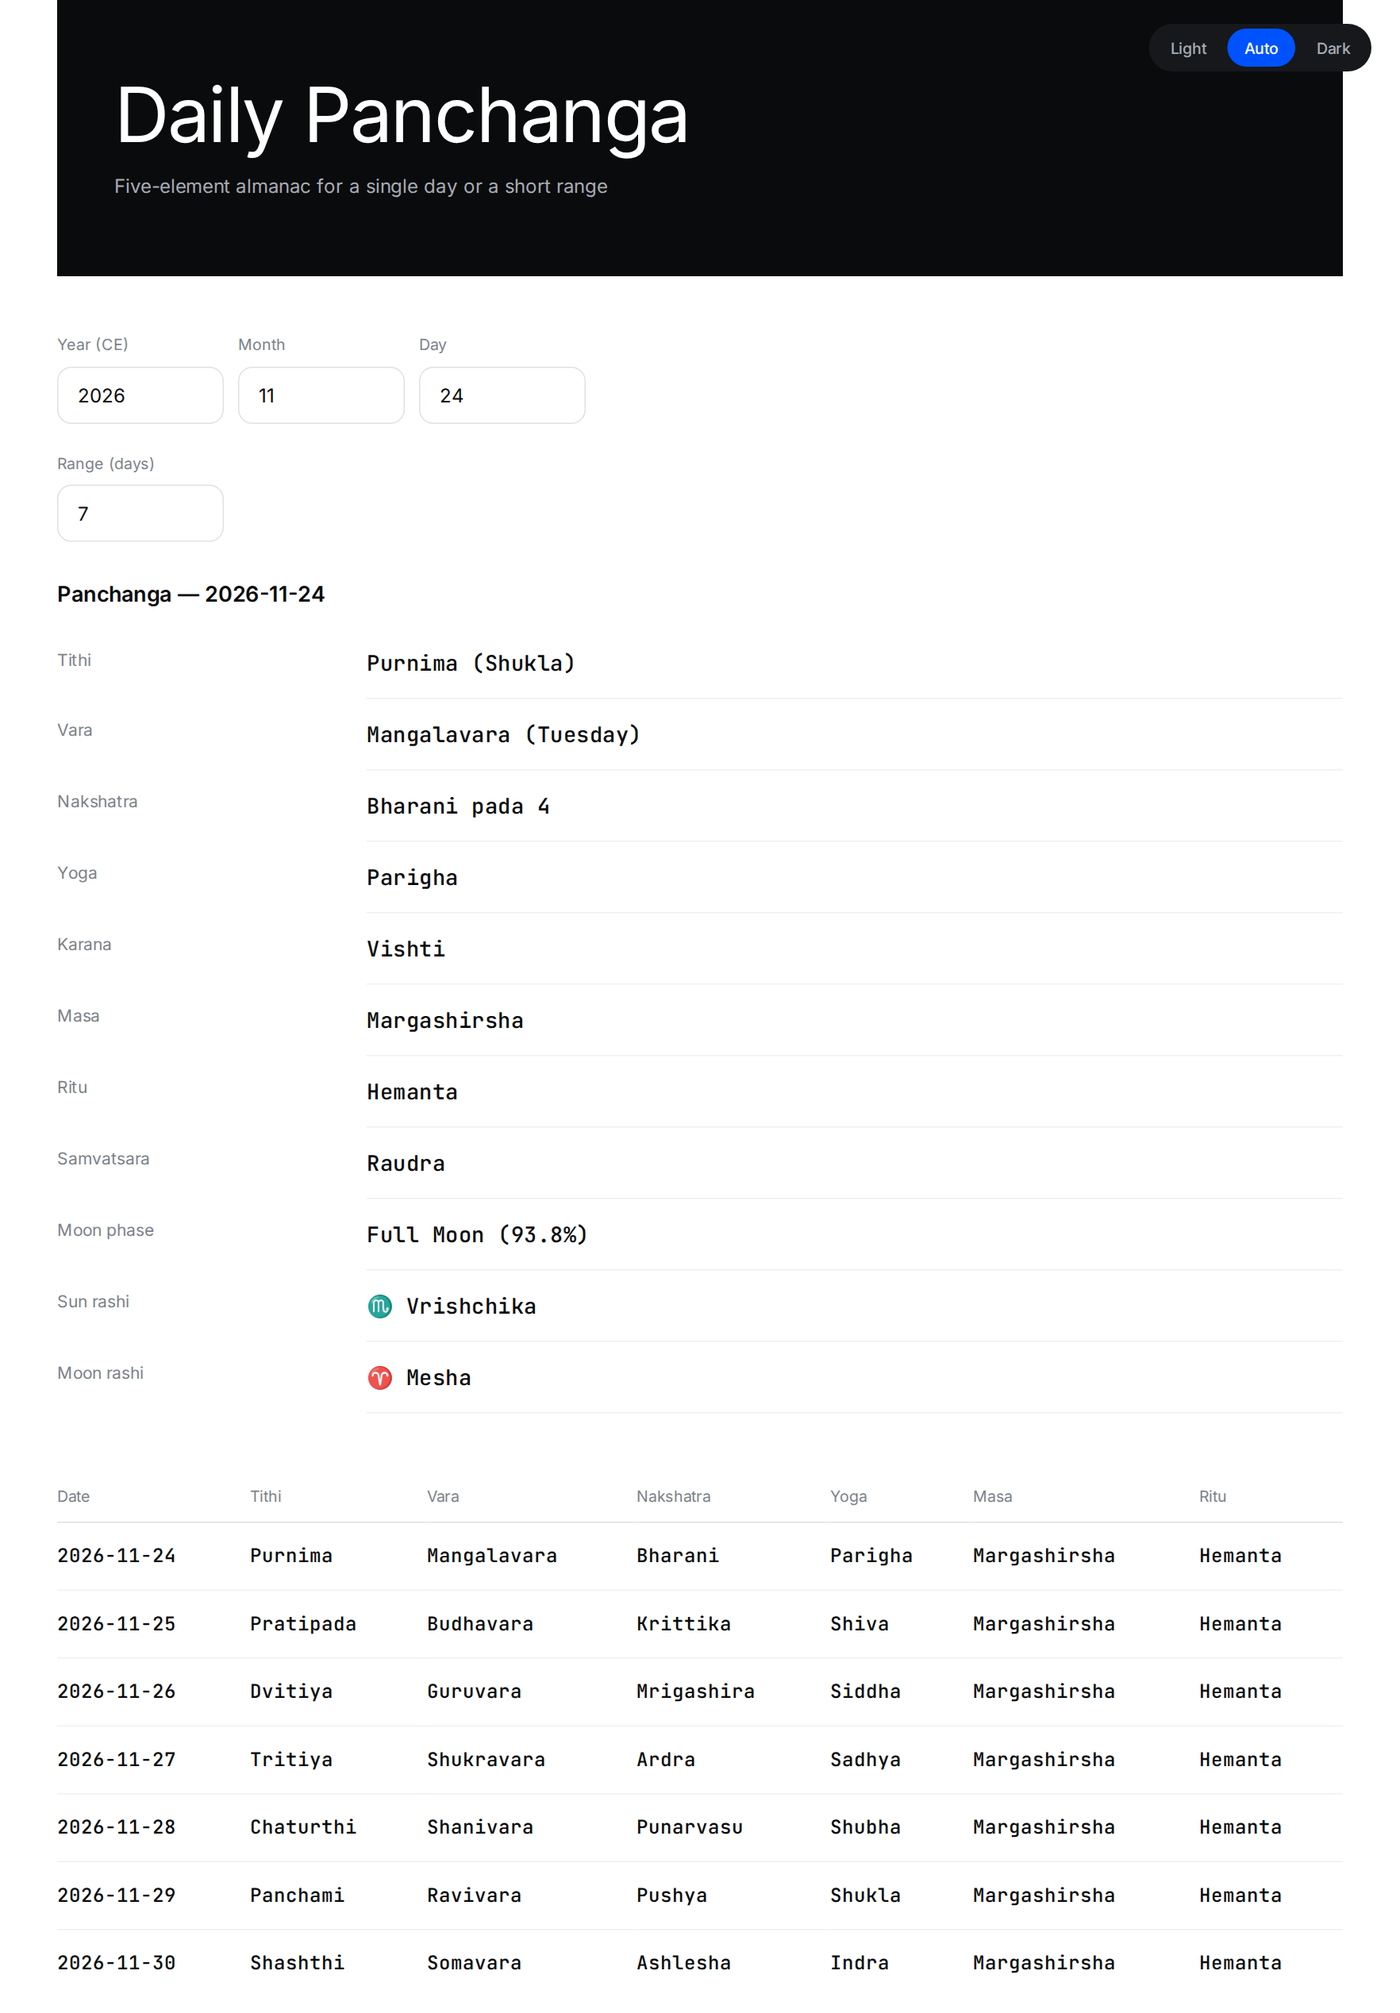
\includegraphics[width=\linewidth,height=0.62\textheight,keepaspectratio]{ui/ui-daily-panchanga.png}
  \caption{Daily Panchanga card and seven-day range}
  \label{fig:ui-daily-panchanga}
\end{figure}

\subsection{Surya Siddhanta AI panel}

The ``Surya Siddhanta AI'' link under the AI heading opens the side
panel, which can also be opened from a floating button. On wide
screens the panel stays open by default and remembers whether the user
closed it. It has two tabs.

\textbf{AI Chat} takes a question in plain language, for example
``When is the next lunar eclipse?'' or ``What does verse 2.39 say?''.
With each question the page sends the user's clock time, time zone and
place, so that ``today'' or ``tomorrow'' is resolved for that user.
Each answer can be expanded to show the calculation tools the assistant
called and is followed by citation chips that mark each source as a
Burgess verse or as commentary. A failed request can be retried and
``New chat'' clears the conversation on the server. Section~\ref{sec:corpus-chatbot}
explains how the answers are grounded.

\begin{figure}[htbp]
  \centering
  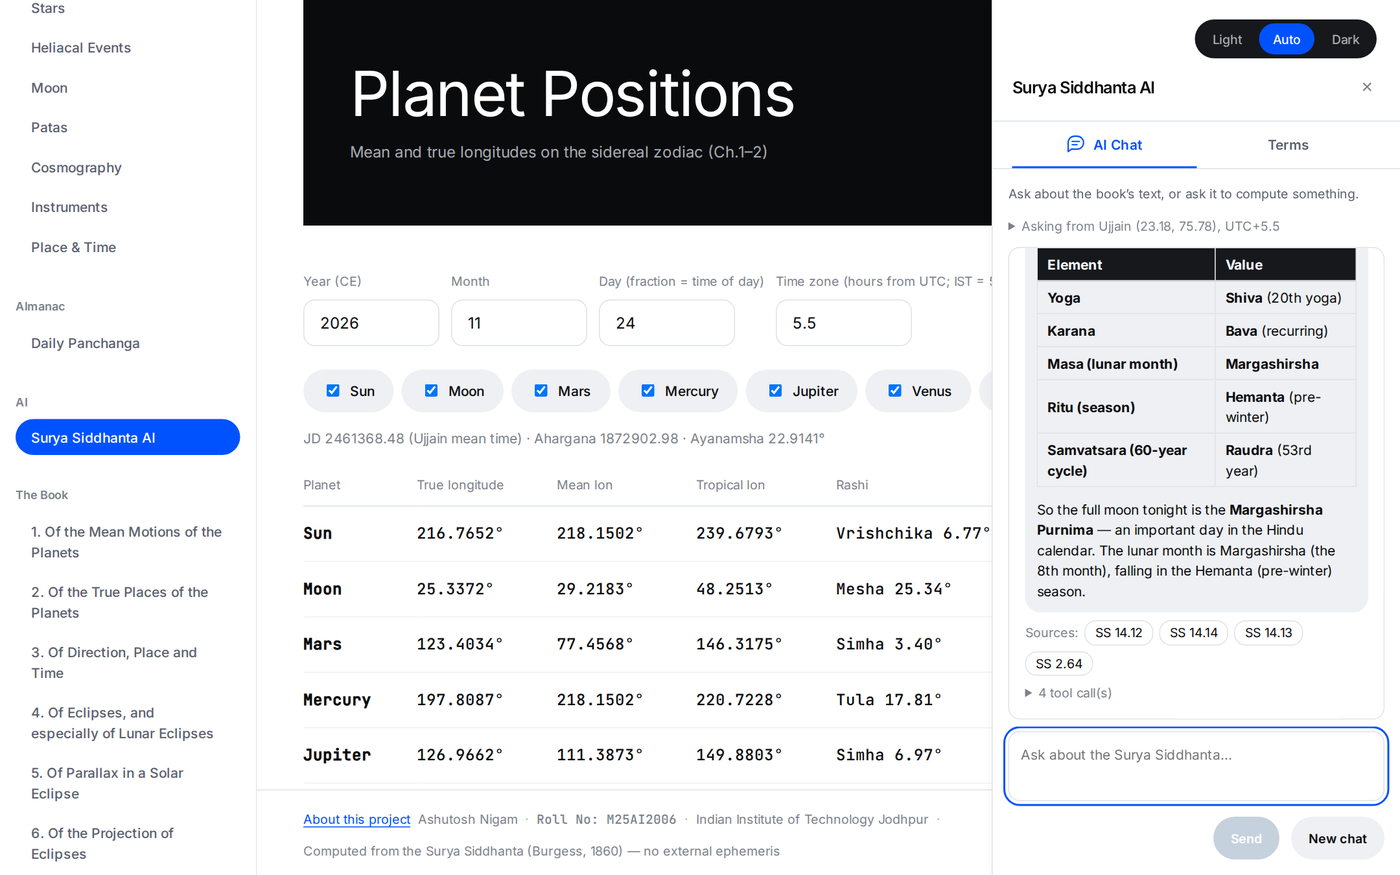
\includegraphics[width=\linewidth,height=0.62\textheight,keepaspectratio]{ui/ui-chat.png}
  \caption{AI Chat answering a question, with source chips and the tool-call list}
  \label{fig:ui-chat}
\end{figure}

\textbf{Terms} is the glossary. It scans the page being viewed and
lists the Sanskrit and technical terms it finds under ``On this page'',
with other related terms under ``Also mentioned''. A filter box
narrows the list. Choosing a term opens a dialog with its definition,
the verses where it occurs and related terms.

\begin{figure}[htbp]
  \centering
  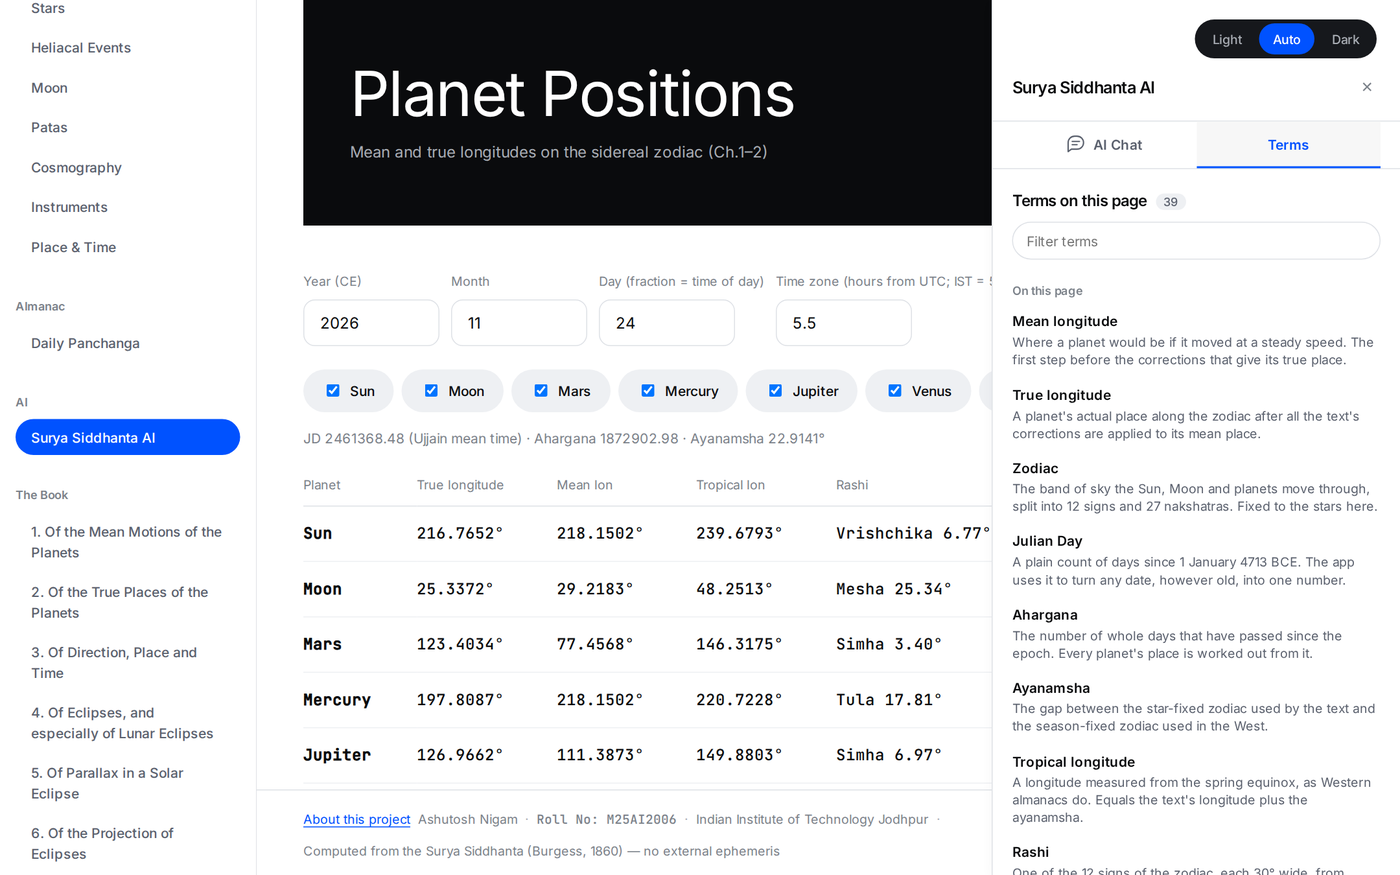
\includegraphics[width=\linewidth,height=0.62\textheight,keepaspectratio]{ui/ui-terms.png}
  \caption{Terms tab listing the glossary terms found on the current page}
  \label{fig:ui-terms}
\end{figure}

\subsection{The Book menu}

The last sidebar group lists the fourteen chapters by Burgess's titles,
from ``Of the Mean Motions of the Planets'' to ``Of the Different
Modes of Reckoning Time''. Each chapter page opens with a short
introduction and the inputs that chapter needs: a date for every
chapter, a place for chapters that depend on the observer (5, 6, 8, 10, 12
and 13), a pair of bodies for Chapter 7, a planet for Chapter 9, a
search window for Chapter 11, a gnomon shadow for Chapter 13 and a
unit conversion and Jupiter-cycle method for Chapter 14. The page is
then a sequence of verse cards. Each card shows the verse number and a
title, one line saying what the verse computes, the verse text with
its corpus citation, and the verse's own calculation for the chosen
inputs. Cards whose result does not change with the date are marked as
such. Where the text's method and the library's method differ, both
results are shown side by side. If the corpus cannot be reached, the
cards still compute and say that the verse text is missing. The page
also notes which verses of the chapter are not laid out as cards.

\begin{figure}[htbp]
  \centering
  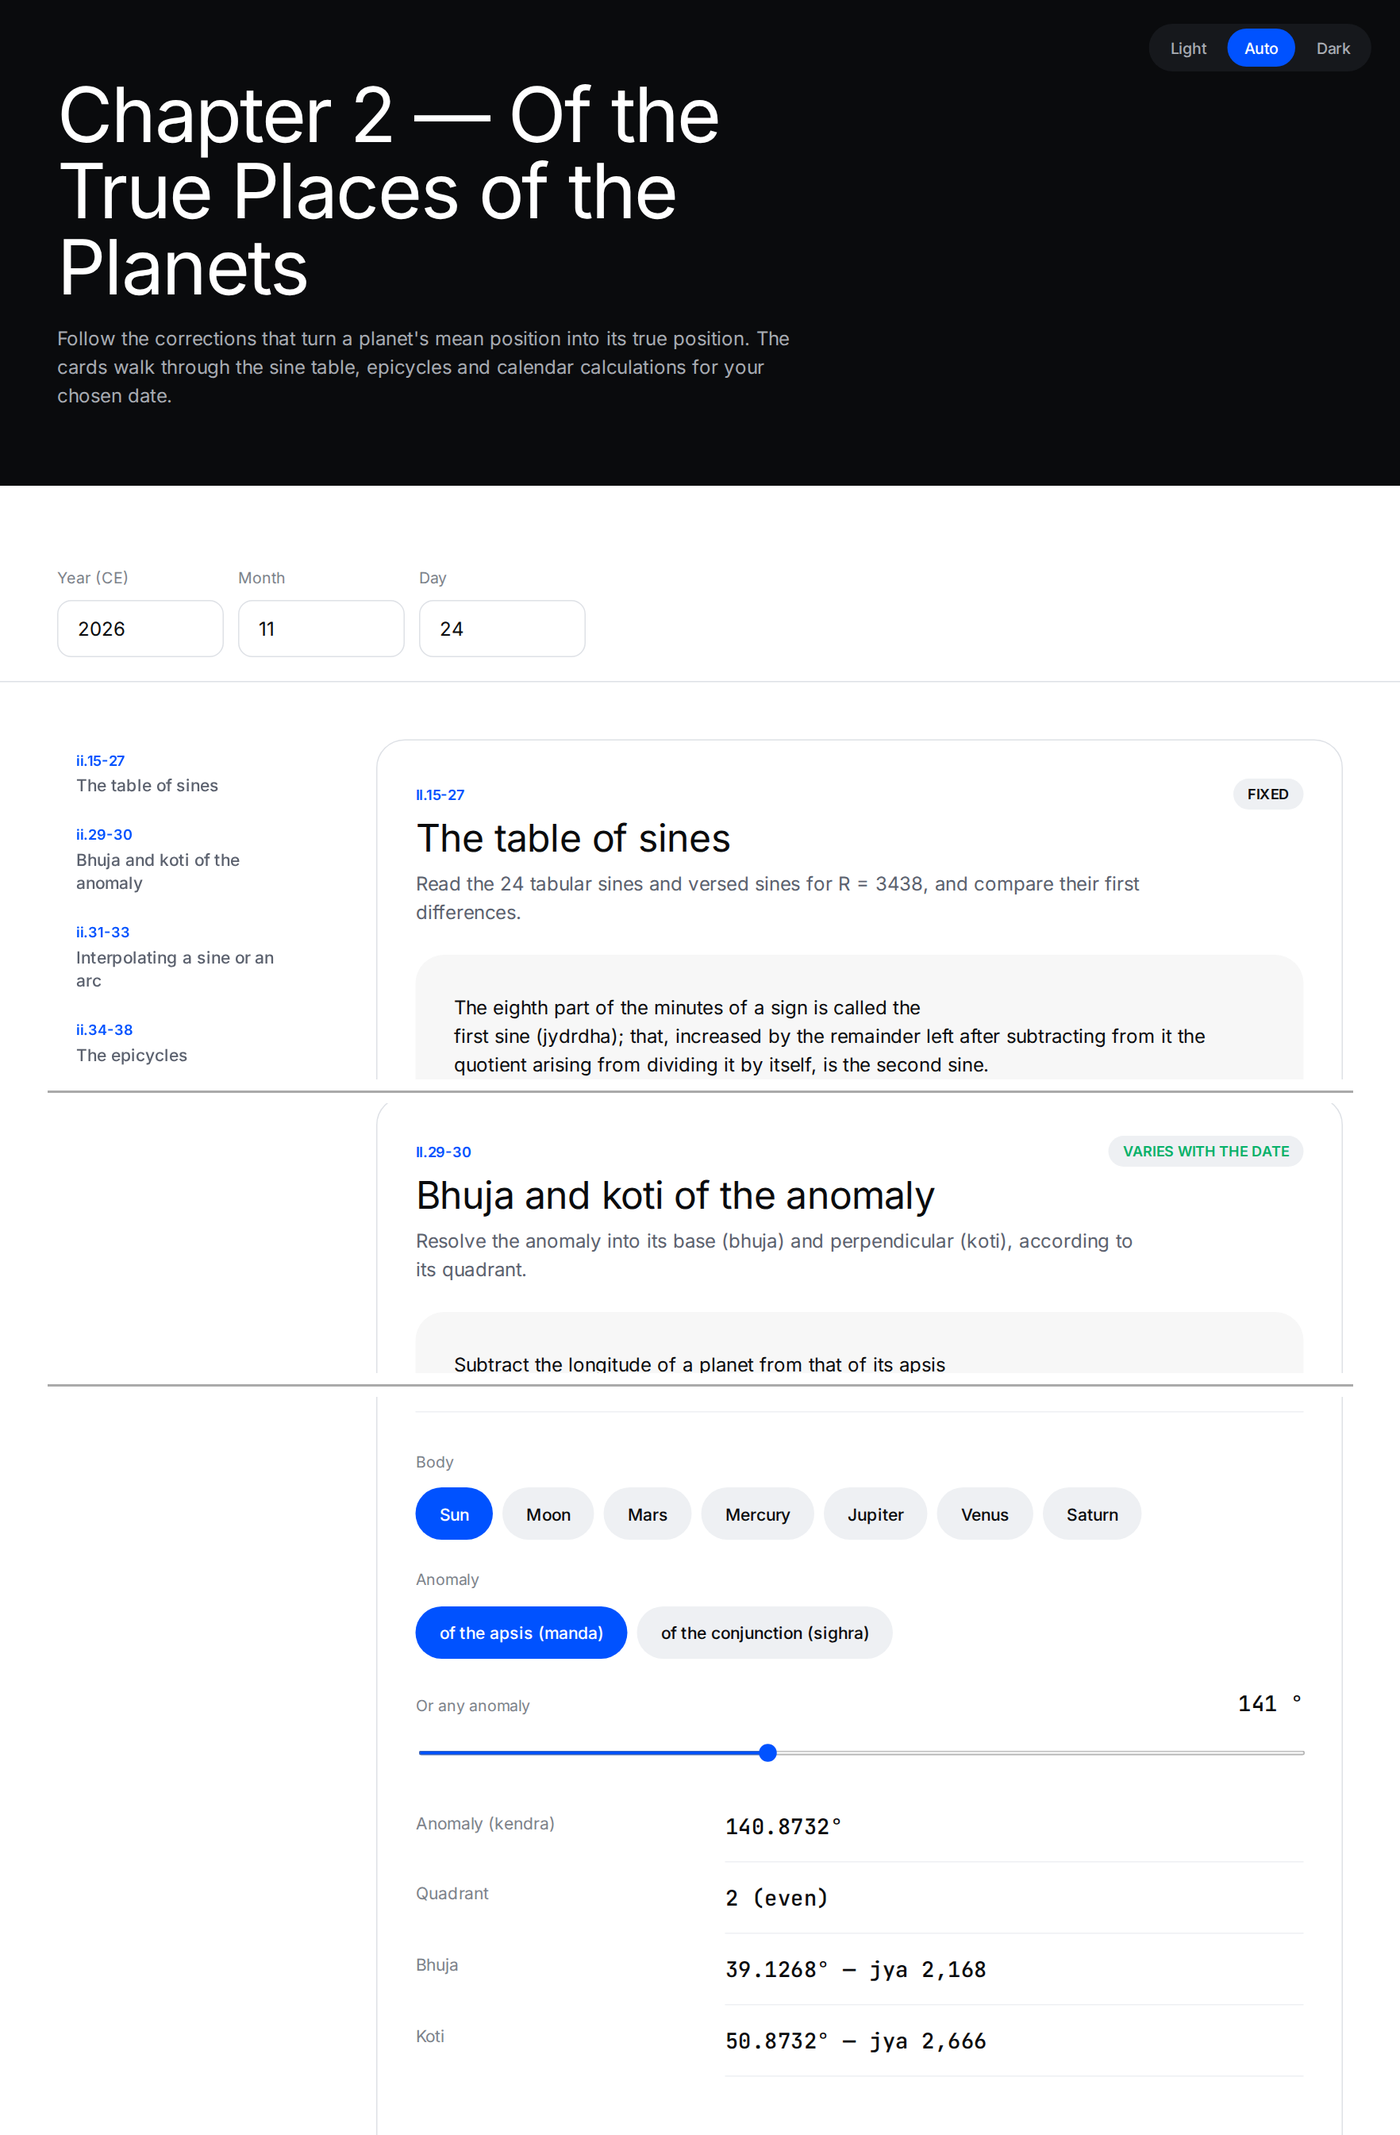
\includegraphics[width=\linewidth,height=0.62\textheight,keepaspectratio]{ui/ui-book.png}
  \caption{Book page for Chapter 2: header, date input, verse index and two verse cards (the cut lines mark omitted parts of the page)}
  \label{fig:ui-book}
\end{figure}

\chapter{Results And Findings}

\section{Worked-Examples Case Studies}

We found that a program may run successfully even when the astronomical formula has been interpreted incorrectly. We observed this while implementing the inner-planet corrections for Mercury and Venus. In our initial implementation, we used the \emph{śīghrocca} revolution counts as their mean planetary motions, which caused the calculated \emph{śīghra} anomaly to become zero. On one test date, we obtained an angular separation of approximately 153° between Mercury and the Sun, which is not reasonable for an inner planet. We identified this error using an elongation limit check. We also found an issue in the \emph{manda} correction, where the anomaly was calculated using the wrong sign convention. Reversing the direction between the apsis and the planetary longitude changed the calculated solar position by several degrees.

We identified another problem while testing a worked solar-eclipse example for Kashi. In our initial implementation, we mixed Ujjain local time and Universal Time during the calculation. This produced a longitude parallax correction of 3.83 \emph{ghaṭikās}, whereas Srivastava's worked example gives 1.06~\cite{shrivastava} \emph{ghaṭikās}. After applying a consistent time convention, we reduced the calculated value to 1.16 \emph{ghaṭikās}. The remaining difference of 0.10 \emph{ghaṭikā} may be related to the iterative procedure and the treatment of apparent disc size in the commentary. Through this example, we found that checking intermediate values and source-specific calculation methods is important rather than comparing only the final results.

We also found an error while calculating the Moon's apparent diameter. Our earlier implementation used an incorrect scaling rule that predicted the largest apparent lunar diameter at apogee. We corrected this by following the verse-based method, which scales the mean diameter using the ratio of true daily motion to mean daily motion. Comparing the intermediate values with the worked example helped us identify and correct the error.

We performed additional validation using the calculations from Chapters 12 and 14. In Chapter 12, we found that the orbital values calculated using the common-distance rule closely agreed with the values printed in the text. This provided an internal consistency check for our implementation. In Chapter 14, we added tests to detect off-by-one errors in season names and Jovian year names. After correcting the identified issues, we also added specific regression tests to detect similar errors during future code changes. Through these case studies, we found that a single verification method is not sufficient. We used domain-specific limits, worked numerical examples, intermediate values and cross-chapter consistency checks to identify different types of calculation errors.

\section{DE440 Evaluation}
\label{sec:de440}

We also carried out a companion study~\cite{nigam2026de440} to compare the longitude calculations from Chapters 1 and 2 of the \emph{\surya} with the modern JPL DE440 ephemeris~\cite{Park2021DE440}. We compared the Sun, Moon, five visible planets and the lunar node using 40,176 sample epochs at ten-day intervals from 1550 to 2649 CE. We used two different time treatments for this comparison. The first method directly uses the library's Julian Date as the reference time, while the second applies corrections for the Ujjain meridian and approximate ΔT. We independently revalidated all 642,816 stored residual values using the local DE440~\cite{Park2021DE440} kernel~\cite{jplephem,acton1996} and found agreement within approximately 0.00000055°. This confirmed that the stored residual calculations were arithmetically consistent with the selected coordinate-frame and time conventions. However, this validation does not establish that every interpretation of the original verses is correct. It also does not validate event predictions from later chapters or historical Panchanga practices.

For the comparison with DE440~\cite{Park2021DE440}, we converted the sidereal longitudes calculated by our library into tropical longitudes by adding the ayanamsha value used in the project. We then calculated the longitude differences against the modern reference positions. The precession-corrected residual used in our study is a scalar longitude comparison and does not represent a complete three-dimensional coordinate-frame transformation. We also observed that the trepidation model reaches its maximum around 2299 CE and then begins to reverse. This behaviour affects the calculated positions when the historical model is extended to future dates. We maintained a revalidation note in the repository that records concerns identified during an earlier review in October 2026. These findings need to be considered with respect to the code revision available at that time. To make the study reproducible, we also provided the regenerate\_paper.py script and REPRODUCE.md instructions in the GitHub repository~\cite{nigam_repo}. The Research Explorer displays the previously calculated results rather than rerunning the complete DE440~\cite{Park2021DE440} comparison or independently estimating the model coefficients.

We selected the study period within the time coverage of the local DE440~\cite{Park2021DE440} kernel. For the modern reference calculations, we used geometric geocentric vectors and converted them to the mean ecliptic and equinox of date~\cite{capitaine2003,hilton2006} before comparing the longitudes. We also handled angular wrapping to avoid incorrect differences near the 0° and 360° boundaries. The lunar node required a different treatment because we derived its reference direction from the Moon's orbital angular momentum. Therefore, its longitude residual has a different physical meaning from the residuals calculated for the planets. We included future dates mainly to examine how the historical constants and trepidation model behave over long periods. These results represent model extrapolations and should not be considered future observations. In the Research Explorer, we grouped the saved decimal-year samples into the same time periods used in the study tables and checked the exported results against the stored values.

During an earlier revalidation, we identified twelve sample epochs whose decimal-year labels placed them in incorrect century groups. This showed us that verifying the numerical residuals alone was not sufficient because errors could also occur while grouping and presenting the results. We therefore added separate tests for the Research Explorer. These tests verify all 176 combinations of celestial body, time period and time-treatment method against the current saved tables. We also check the source hashes, sample coverage and retained minimum and maximum values. These checks help us confirm that the explorer presents the stored results consistently. However, they do not independently repeat the DE440~\cite{Park2021DE440} calculations or validate the timing of astronomical events. We also recognise that longitude and elongation errors cannot be directly treated as eclipse or tithi timing errors without separately calculating and validating the corresponding event times.

\section{Interface Validation and Reproducibility}

We reviewed the verification records. These are maintained in the GitHub repository~\cite{nigam_repo}. The verification record of 8 November 2026 reports that 1,677 tests passed successfully after the corpus repair using the command PYTHONPATH=src python -m pytest -q~\cite{pytest}. The learning-path validation record dated 4 November 2026 reports 1,653 passing tests. The same record also includes an earlier focused run of 49 tests covering test\_learning\_lab\_data.py, test\_research\_explorer\_data.py and test\_api\_book\_ch02.py, along with a successful production build of the frontend.

We obtained these results by running it multiple times and then fetched from the dated verification records available in the repository. We did not execute the tests again while preparing this version of the report. Therefore, the reported test counts represent the results of those recorded runs and should not be considered a new verification of the current codebase.

\begin{longtable}[]{@{}
  >{\raggedright\arraybackslash}p{(\linewidth - 2\tabcolsep) * \real{0.5000}}
  >{\raggedright\arraybackslash}p{(\linewidth - 2\tabcolsep) * \real{0.5000}}@{}}
\caption{Interface validation checks and their evidence}\label{tab:validation}\\
\toprule\noalign{}
Check & Evidence \\
\midrule\noalign{}
\endfirsthead
\caption[]{Interface validation checks and their evidence (continued)}\\
\toprule\noalign{}
Check & Evidence \\
\midrule\noalign{}
\endhead
\bottomrule\noalign{}
\endlastfoot
Source-data integrity & All 176 body-window-treatment groups match the saved tables; each body has 40,176 samples per treatment. \\
Aggregation and provenance & Source hashes, complete sample counts, RMS, signed means and sampled extrema are checked; generated files must match fresh exports. \\
Browser workflows & Real API values, correction stages, whole-day stepping, date-preserving links, rapid responses, failure/retry, optional corpus, understanding feedback and exports. \\
Research interaction & 88 matrix cells; all 16 body/treatment combinations; JSON and CSV metadata; keyboard selection and mobile overflow checks. \\
Visual review & Light and dark desktop layouts and a 390-pixel mobile layout; screenshot evidence retained with the project. \\
\end{longtable}

We also developed two frontend data export scripts, \path{docs/evaluation/export_learning_lab.py} and export\_research\_explorer.py, to support the reproducibility of the Learning Lab and Research Explorer results. These scripts process and summarise the saved CSV files without generating new DE440~\cite{Park2021DE440} reference positions. We documented the complete procedure for reproducing the original comparison study separately in \path{docs/evaluation/REPRODUCE.md}.

We also added browser-level tests~\cite{playwright} for all eight learning lessons and the Research Explorer. These tests check the API responses, lesson evidence exports, lunar node geometry, quiz functionality, source links that retain the selected date, handling of outdated API responses, retry behaviour and mobile layouts. We also verified that the calculation features remain available when the optional corpus text is missing.

Through these tests, we checked whether the implemented software behaves as expected under different conditions. However, these results do not independently establish the historical authenticity of the implemented astronomical rules, the accuracy of eclipse timing or the educational effectiveness of the learning features. These aspects require separate validation methods and further evaluation.

\section{Implementation Size}

We inspected the source code on 13 November 2026 to count the registered API operations and the locations where tables are rendered in the application. We used these counts to describe the size and scope of our implementation. However, these numbers do not directly represent the numerical accuracy of the calculations, the extent of test coverage or the number of tables visible to users on a single screen.

\begin{longtable}[]{@{}
  >{\raggedright\arraybackslash}p{(\linewidth - 2\tabcolsep) * \real{0.2632}}
  >{\raggedright\arraybackslash}p{(\linewidth - 2\tabcolsep) * \real{0.7368}}@{}}
\caption{API and frontend inventory}\label{tab:inventory}\\
\toprule\noalign{}
\textbf{Measure} & \textbf{Count and definition} \\
\midrule\noalign{}
\endfirsthead
\caption[]{API and frontend inventory (continued)}\\
\toprule\noalign{}
\textbf{Measure} & \textbf{Count and definition} \\
\midrule\noalign{}
\endhead
\bottomrule\noalign{}
\endlastfoot
Backend API endpoints & 56 method-and-path operations: 46 POST and 10 GET. This includes 54 application operations, the service index and the health check. Automatically generated documentation routes are excluded. \\
Frontend table placements & 167 static JSX render locations: 103 KVTable uses, 58 GridTable uses and 6 direct HTML tables. The two reusable table definitions are excluded. \\
Counting basis & FastAPI app.openapi() for endpoints~\cite{fastapi}; the TypeScript compiler AST~\cite{typescript} for frontend/src TSX files. The figures describe the checkout inspected on 13 November 2026, not a benchmark. \\
\end{longtable}

A table location in the source code may be conditional, and the same component can also render a table multiple times when it is reused or repeated in a loop. Therefore, this count should not be treated as the number of unique datasets, database tables, or tables visible at the same time.

\chapter{Summary And Future Plan Of Work}

\section{Summary of Completed Work}

We developed a reusable Python calculation library that covers the computable astronomical procedures from all fourteen chapters of the \emph{\surya}. Along with the calculation library, we implemented source-text processing, verse retrieval and multiple user interfaces. We organised the calculation functions so that they can be accessed through both chapter-based and planet-based modules. The corpus allows users to examine the textual rules associated with the calculations, while the AI assistant uses calculation and retrieval tools to answer user questions. We also developed eight learning paths, the Universe Explorer and the Research Explorer to help users study and understand the astronomical calculations through different interfaces. During development, we used worked numerical examples to identify and correct several errors related to the interpretation of astronomical rules and time conventions. We also compared the calculated planetary longitudes with the modern JPL DE440 ephemeris~\cite{Park2021DE440,nigam2026de440} to measure the differences between the historical model and modern reference positions under defined assumptions and coordinate conventions.

We maintained the Hindi OCR and translation work separately from the English verse corpus currently included in the application. This distinction helps us keep the source-processing work organised and avoids presenting the Hindi and English materials as a fully aligned corpus when that integration has not yet been completed.

\section{Limitations and Next Work}

We implemented the computable astronomical procedures from all fourteen chapters of the \emph{\surya}, but not every verse could be converted into a numerical calculation. So we documented the remaining limitations in the computational-edition manuscript~\cite{nigam2026edition}. These include complete iterative eclipse calculations, some rules related to apparent disc diameter and visibility, parts of the equation of time and descriptive passages that do not provide complete numerical procedures. Although the bundled Burgess corpus contains all numbered verses, some OCR errors still remain. The optional external commentary also requires further verification. We documented our interpretations of star coordinates and procedures reconstructed with the help of commentary. These should be considered implementation choices rather than the only possible historical interpretations. We also used modern trigonometric functions in our calculations, so the results may not reproduce every intermediate rounding step used in historical manual calculations.

In future work, we plan to preserve the worked-example verification results with a fixed code revision and independently rerun the complete DE440~\cite{Park2021DE440} comparison pipeline. We also aim to extend the implementation wherever the original text or commentary provides a sufficiently clear calculation procedure. The Hindi OCR and translation material requires further review and verse-level alignment before it can be integrated with the English corpus as a reliable bilingual resource. Our eight learning paths currently cover the Sun, Moon, five classical planets and Rahu. Although we developed these activities to support learning, we have not yet conducted a student study to measure their educational effectiveness. Such a study would be required to determine whether these features improve students' understanding of the astronomical concepts.

We recognise that the \emph{\surya} contains both computational rules and descriptive material. Implementing every verse as a software function would require introducing numerical assumptions that may not be supported by the original text. Therefore, we limited our implementation to the computable procedures across all fourteen chapters and documented the remaining exceptions. In future versions, we can extend the eclipse calculations by implementing the complete iterative procedure and comparing its intermediate results with Srivastava's worked examples~\cite{shrivastava}. We can also examine alternative interpretations of star coordinates and compare their calculated results with the existing implementation. The modular structure of the library allows us to make and test these changes without modifying unrelated calculations.

We also plan to strengthen the reproducibility of our results. Future changes to eclipse calculations will be checked against the intermediate values provided in the commentary, while alternative star-coordinate methods will be evaluated through direct numerical comparisons. We will verify corpus corrections against the original scanned pages and maintain fixed versions of the corrected texts. We also plan to regenerate the DE440~\cite{Park2021DE440} comparison tables using a recorded code revision and a verified ephemeris kernel. These improvements will help other researchers reproduce our calculations, examine the assumptions used in the implementation and investigate the remaining differences between the historical methods and modern astronomical results.

\cleardoublepage
\phantomsection
\addcontentsline{toc}{chapter}{References}
\renewcommand{\bibname}{References}
\nocite{pyswisseph}
\bibliographystyle{unsrtnat}
\bibliography{references}

\end{document}
